\documentclass[10pt,letterpaper]{article}
\usepackage[top=0.85in,left=2.75in,footskip=0.75in]{geometry}
\usepackage{amsmath,amssymb}
\usepackage{changepage}
\usepackage[utf8x]{inputenc}
\usepackage{textcomp,marvosym}
\usepackage{cite}
\usepackage{nameref,hyperref}
\usepackage[right]{lineno}
\usepackage{microtype}
\usepackage[table]{xcolor}
\usepackage{array}
\newcolumntype{+}{!{\vrule width 2pt}}

% create \thickcline for thick horizontal lines of variable length
\newlength\savedwidth
\newcommand\thickcline[1]{%
  \noalign{\global\savedwidth\arrayrulewidth\global\arrayrulewidth 2pt}%
  \cline{#1}%
  \noalign{\vskip\arrayrulewidth}%
  \noalign{\global\arrayrulewidth\savedwidth}%
}

% \thickhline command for thick horizontal lines that span the table
\newcommand\thickhline{\noalign{\global\savedwidth\arrayrulewidth\global\arrayrulewidth 2pt}%
\hline
\noalign{\global\arrayrulewidth\savedwidth}}


% Remove comment for double spacing
%\usepackage{setspace}
%\doublespacing

% Text layout
\raggedright
\setlength{\parindent}{0.5cm}
\textwidth 5.25in
\textheight 8.75in

% Bold the 'Figure #' in the caption and separate it from the title/caption with a period
% Captions will be left justified
\usepackage[aboveskip=1pt,labelfont=bf,labelsep=period,justification=raggedright,singlelinecheck=off]{caption}
\renewcommand{\figurename}{Fig}

% Use the PLoS provided BiBTeX style
\bibliographystyle{plos2015}

% Remove brackets from numbering in List of References
\makeatletter
\renewcommand{\@biblabel}[1]{\quad#1.}
\makeatother



% Header and Footer with logo
\usepackage{lastpage,fancyhdr,graphicx}
\usepackage{epstopdf}
%\pagestyle{myheadings}
\pagestyle{fancy}
\fancyhf{}
%\setlength{\headheight}{27.023pt}
%\lhead{\includegraphics[width=2.0in]{PLOS-submission.eps}}
\rfoot{\thepage/\pageref{LastPage}}
\renewcommand{\headrulewidth}{0pt}
\renewcommand{\footrule}{\hrule height 2pt \vspace{2mm}}
\fancyheadoffset[L]{2.25in}
\fancyfootoffset[L]{2.25in}
\lfoot{\today}

%% Include all macros below

\newcommand{\lorem}{{\bf LOREM}}
\newcommand{\ipsum}{{\bf IPSUM}}

%% extra packages
\usepackage{caption}
\usepackage{subcaption}

%% END MACROS SECTION


\begin{document}
\vspace*{0.2in}

% Title must be 250 characters or less.
\begin{flushleft}
{\Large
\textbf\newline{Galaxy Training: A Powerful Framework for Teaching} 
}
\newline
% Insert author names, affiliations and corresponding author email (do not include titles, positions, or degrees).
\\
\color{blue} \textbf{NOTE: please add your name and affiliation below if you want to be on this paper! This project is only possibly because of the amazing community behind it. If you have contributed in any way to this project, you may add yourself as an author. (And contributions come in many forms, GitHub contributions are just one form, and not a requirement). } \\
\color{black}
\ \\
Saskia Hiltemann\textsuperscript{1\Yinyang\textpilcrow},
Helena Rasche\textsuperscript{1,15,2\Yinyang},
Simon Gladman \textsuperscript{3},
Hans-Rudolf Hotz \textsuperscript{4},
Delphine Larivière \textsuperscript{5},
Daniel Blankenberg \textsuperscript{6},
Pratik D. Jagtap \textsuperscript{7},
Thomas Wollmann \textsuperscript{8},
Anthony Bretaudeau \textsuperscript{9,10},
Nadia Goué \textsuperscript{11},
Timothy J. Griffin \textsuperscript{7},
Coline Royaux\textsuperscript{12},
Yvan Le Bras\textsuperscript{12},
Subina Mehta\textsuperscript{7},
Anna Syme\textsuperscript{3},
Frederik Coppens\textsuperscript{13,14},
Bert Droesbeke\textsuperscript{13,14},
Nicola Soranzo\textsuperscript{16},,
\color{blue}Add your name here\textsuperscript{15}\color{black},
Björn Grüning \textsuperscript{2\ddag}
Bérénice Batut\textsuperscript{2\ddag},
with the GTN community
\\
\bigskip
\textbf{1} Clinical Bioinformatics Group, Department of Pathology, Erasmus Medical Center, Wytemaweg 80, 3015 CN, Rotterdam, The Netherlands \\
\textbf{2} Bioinformatics Group, Department of Computer Science, Albert-Ludwigs-University Freiburg, Georges-Köhler-Allee 106, Freiburg 79110, Germany \\
\textbf{3} Melbourne Bioinformatics, University of Melbourne, Parkville, Victoria, Australia \\
\textbf{4} Friedrich Miescher Institute for Biomedical Research, Basel, Switzerland and SIB Swiss Institute of Bioinformatics, Basel, Switzerland \\
\textbf{5} Eberly College of Science, Pennsylvania State University, State College, U.S.A. \\
\textbf{6} Genomic Medicine Institute, Lerner Research Institute, Cleveland Clinic, Cleveland, OH, USA  \\
\textbf{7} Department of Biochemistry, Molecular Biology and Biophysics, University of Minnesota, Minneapolis, MN, USA  \\
\textbf{8} Biomedical Computer Vision Group, BioQuant, IPMB, Heidelberg University\\ Im Neuenheimer Feld 267, Heidelberg, Germany. \\
\textbf{9} IGEPP, INRAE, Institut Agro, Univ Rennes, 35000, Rennes, France.\\
\textbf{10} GenOuest Core Facility, Univ Rennes, Inria, CNRS, IRISA, 35000, Rennes, France.\\
\textbf{11} AuBi, Mésocentre, Clermont Auvergne University, 63178, Aubière, France.\\
\textbf{12} PNDB French Biodiversity e-infrastructure, UMS PatriNat, French Museum of Natural History, 29900, Concarneau, France.\\
\textbf{13} Department of Plant Biotechnology and Bioinformatics, Ghent University, Technologiepark 71, Ghent 9052, Belgium.\\
\textbf{14} VIB Center for Plant Systems Biology, Technologiepark 71, Ghent 9052, Belgium.\\
\textbf{15} Academie voor de Technologie van Gezondheid en Milieu, Avans Hogeschool, Lovensdijkstraat 63, 4818 AJ Breda, the Netherlands.\\
\textbf{16} Earlham Institute, Norwich Research Park, Norwich, NR4 7UZ, UK.\\
\color{blue}\textbf{14} AddYoursHere! Affiliation Dept/Program/Center, Institution Name, City, State, Country \color{black}\\
%TODO: add your affiliation here as needed
\bigskip

% Insert additional author notes using the symbols described below. Insert symbol callouts after author names as necessary.
%
% Remove or comment out the author notes below if they aren't used.
%
% Primary Equal Contribution Note
\Yinyang These authors contributed equally to this work.

% Additional Equal Contribution Note
% Also use this double-dagger symbol for special authorship notes, such as senior authorship.
\ddag These authors also contributed equally to this work.

% Current address notes
%\textcurrency Current Address: Dept/Program/Center, Institution Name, City, State, Country % change symbol to "\textcurrency a" if more than one current address note
% \textcurrency b Insert second current address
% \textcurrency c Insert third current address

% Deceased author note
%\dag Deceased

% Group/Consortium Author Note
\textpilcrow Membership list can be found in the Acknowledgments section.

% Use the asterisk to denote corresponding authorship and provide email address in note below.
* saskiahiltemann@gmail.com

\end{flushleft}


% Please keep the abstract below 300 words
\section*{Abstract}
There is an ongoing explosion of scientific datasets being generated, brought on by recent technological advances in many areas of the natural sciences.
As a result, the life sciences have become increasingly computational in nature, and bioinformatics has taken on a central role in research studies.
However, basic computational skills and data analysis and stewardship are still rarely taught in life science educational programs \cite{Attwood2019}, resulting in a skills gap in many of the researchers tasked with analysing these big datasets.
In order to address this skills gap and empower researchers to perform their own data analyses, the Galaxy Training Network (GTN) developed the Galaxy Training Platform (\url{https://training.galaxyproject.org}) in 2016; an open access, community-driven framework for the collection of training materials for data analysis, utilizing the web-based user-friendly Galaxy data analysis platform.

Since its inception, this training platform has thrived, with the number of tutorials and contributors growing rapidly, and the range of topics extending beyond life sciences to include topics such as climatology, cheminformatics and machine learning.
While initially aimed at supporting researchers directly, the GTN framework has proven to be an invaluable resource for educators as well. We have focused our efforts in recent years on adding increased support for this growing community of instructors.
We have added features aimed at facilitating the use of the materials in a classroom setting, simplifying the contribution flow for new materials, and adding a set of train-the-trainer lessons.
Here, we present the latest developments in the project, aimed at facilitating the use of the Galaxy Training materials by educators.


% Please keep the Author Summary between 150 and 200 words
% Use first person. PLOS ONE authors please skip this step.
% Author Summary not valid for PLOS ONE submissions.
\section*{Author summary}
The Galaxy Training Network (GTN) comprises an active community of trainers and a diverse set of training materials for the web-based Galaxy data analysis platform. The training material covers a wide range of topics from the natural sciences, and reduces the hurdles to offer the needed training in data analyses on many levels and in different curricula. What once started as a random collection of slide decks used for training, has evolved over the last five years into a well-structured and harmonized platform offering slides, hands-on, tailored datasets, workflows and even interactive tours. 
In this review, we describe the different components of the GTN, we explain how we manage to keep up with the ever changing training requirements while keeping the quality high, and provide evidence how well the GTN is received, both by trainers and trainees. 
%% HRH - it's only ~130 words, but it might be used as a start
%% \emph{We ask that all authors of research articles include a 150–200 word non-technical summary of the work as part of the manuscript to immediately follow the abstract.
%% This text is subject to editorial change, should be written in the first-person voice, and should be distinct from the scientific abstract.
%% Aim to highlight where your work fits within a broader context; present the significance or possible implications of your work simply and objectively; and avoid the use of acronyms and complex terminology wherever possible.
%% The goal is to make your findings accessible to a wide audience that includes both scientists and non-scientists.
%% Authors may benefit from consulting with a science writer or press officer to ensure they effectively communicate their findings to a general audience.}


%\linenumbers

\section*{Introduction}

Education is a fundamental human right (e.g.\ the Universal Declaration of Human Rights (UDHR), the International Covenant on Economic, Social and Cultural Rights (ICESCR)).
Indicators of the achievement of education as a right are outlined in the ICESCR, and further developed into what is known as the “4 As framework” \cite{tomavsevski2001human}, which specifies Availability, Accessibility, Acceptability and Adaptability as essential metrics.
The 4 As, therefore, provide a concrete set of ideals to strive towards in any global educational endeavor.
The goals of the Galaxy project are well aligned with the 4 As.

Galaxy \cite{Jalili2020} is an open source web-based platform for accessible, reproducible, and transparent computational research, driven by an inclusive and diverse worldwide community.
Researchers are able to access a wealth of tools, datasets, and high-performance computing resources through a standard web browser, without requiring informatics expertise. However, they need to learn how to use these resources. A survey of 704 NSF-BIO-funded investigators revealed that training was the top 3 of 13 most unmet needs above HPC/cloud facilities, workflows/pipelines analysis or storage facilities needs, for instance \cite{Barone2017}.

To help solving the need for training, the Galaxy Training Network (GTN; \url{https://training.galaxyproject.org}) benefits from training experiences from e-infrastructures such as Carpentry and ELIXIR. It provides researchers with online training materials, connects them with local trainers, and helps promote open data analysis practices worldwide \cite{Batut2018}. We previously discussed initial support for enabling self-learning using GTN materials, and now explore recent enhancements and capabilities of the framework for short-format training from the educators’ perspective.
The training materials are maintained and community-reviewed in GitHub (\url{https://github.com/galaxyproject/training-material}). They cover an increasing spread of topical domains, such as life sciences, computational chemistry, climatology, data visualization, statistics, and machine learning. 
The resources provided by the GTN have been used to hold more than 100 interactive workshops across the world in 2018-19 alone.
These resources have also been included as part of formal undergraduate and graduate courses. Great effort has been expended to shift the onus of adhering to the FAIR principles \cite{Wilkinson2016} from individual contributors onto the provided public infrastructure, greatly simplifying the creation of robust training materials.
Training Infrastructure as a Service (TIaaS; \cite{Rasche2020}) is available to provide free dedicated compute resources for trainers who are hosting public workshops, but do not have resources of their own. This defect was stressed in \cite{Barone2017} mentioning a CyVerse survey where 58\% of a thousand biologists felt not having the expected computing facilities to carry out their research.
While there is much work to be done, here we illustrate our ongoing efforts to bring availability, accessibility, acceptability and adaptability to bioinformatics education for both trainers and learners alike.


\section*{Results}

The GTN framework and community have grown significantly over the past years. In this section we describe the aims and objectives of this project, showcase some example use-cases, and highlight some of the recent efforts by the GTN community to expand and improve the project. We also present how this project supports both intructors and training material developers.


\subsection*{Galaxy, a platform to support teaching}

Classical hands-on bioinformatics training necessitates that students run bioinformatics software. This software must run somewhere, either on a cluster, installed to a computer lab, or on the learner's private device. By contrast, Galaxy provides access to bioinformatics software requiring only a web browser.

Galaxy \cite{Jalili2020} is an open source, community-driven, and web-based platform for accessible, reproducible, and transparent computational research and training. Complex computational analysis can be performed from a web browser without requiring programming experience or training in high performance computing. It provides access to hundreds of tools ($>$8,000 tools in the ToolShed (\url{https://galaxyproject.org/toolshed/}) as of July 2021) used in a wide variety of analysis areas. Galaxy does all the heavy lifting of installing and managing the software, and provides a user-friendly interface to the end-user. This makes Galaxy the ideal platform for teaching. Students can focus on analytical thinking, tools, and concepts, rather than on details of computational infrastructure. 


Using Galaxy also helps teachers. In one hand, while Galaxy can be installed locally and in the cloud, public servers provide open access to analysis workflows, tools, and reference datasets. So that teachers have access to published data and teach reproducible sciences to students based on published tools and workflows. In other hand, using worldwide public Galaxy servers give access to compute resources: the UseGalaxy.* servers with Galaxy Main (\url{https://usegalaxy.org}), Galaxy Europe (\url{https://usegalaxy.eu}), and Galaxy Australia (\url{https://usegalaxy.org.au}), but also 125+ others (\url{https://galaxyproject.org/use/}). Using one of these public Galaxy servers removes the infrastructure hurdles such as owning and configuring a cluster, or deploying software to machines in a computer lab.

%% During training events, students access Galaxy through the web interface, and thereby have seamless access to thousands of bioinformatics tools.
%% Pre-loaded datasets (aka Galaxy Data Libraries) cut the amount of necessary data transfer.
%% Alternatively, the Galaxy Training Network provides small, but still meaningful, subsampled datasets for the individual training topics.

Over the years, Galaxy has become increasingly attractive as a training platform around the world (Table~\ref{tbl:galaxy_training_stats}). For example, between June 2018 and December 2020, Galaxy Europe server has been used for more than 170 training events reaching more than 5,000 students. Galaxy has been used, as a teaching platform, in a wide range of settings and application domains, as illustrated by the following user stories collected from instructors.

\begin{figure}[!ht]
	\centering
	\begin{subfigure}[b]{0.45\textwidth}
         \centering
         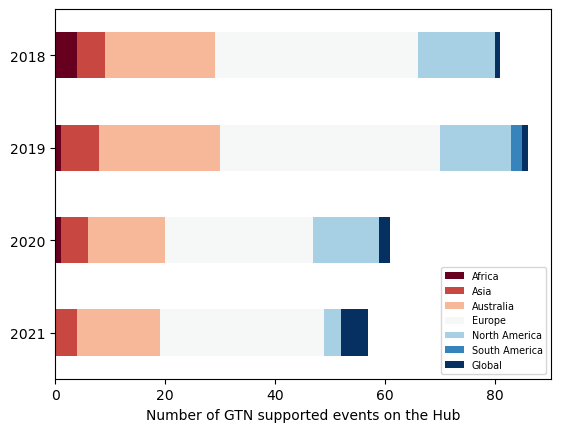
\includegraphics[width=\textwidth]{images/hub-training-per-year.png}
    \caption{Number of events per year and in total since 2018}
         \label{fig:material-evolution}
    \end{subfigure}
    \hfill
    \begin{subfigure}[b]{0.45\textwidth}
         \centering
         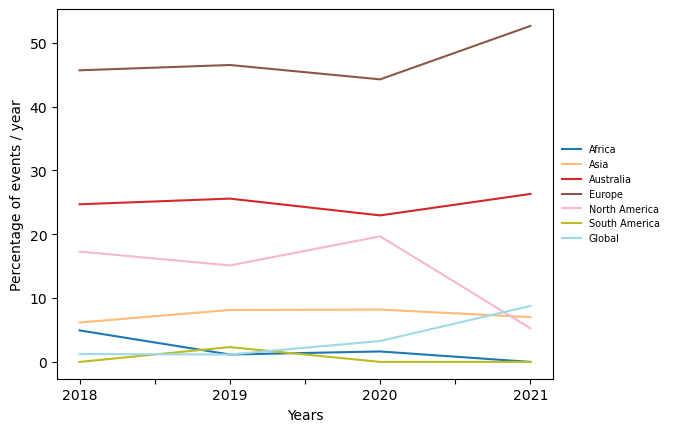
\includegraphics[width=\textwidth]{images/hub-training-over-years.png}
         \caption{Percentage of events per year for each continents (and global)}
         \label{fig:material-number}
    \end{subfigure}
	\caption{Training events supported by GTN materials, registered on the Galaxy Community Hub website (\href{https://galaxyproject.org/}{https://galaxyproject.org/}) over the last 4 years. The Jupyter notebook used to create these figures is available on the GitHub repository for this paper (\url{https://github.com/galaxyproject/GTN-community-paper-2020}) \label{fig:hub-training}}
\end{figure}


\subsubsection*{Graduate Bioinformatics courses}

Galaxy is an integral part of Bioinformatics programs at the undergraduate level (e.g. Clermont Auvergne University, Texas A\&M University, Avans Hogeschool, University of Freiburg). 

In these undergraduate courses, Galaxy is often used to teach the concept of pipelines and workflows, and also reproducibility. Students learn the importance of the tool versions, as tools can change subtly or significantly over time and this may impact their analyses. Teachers can likewise showcase the evolution of algorithms over time using different versions of tools (e.g.\ bowtie and bowtie2) to help students understand the advances in the field. 
Without the need to spend resources on teaching basic Unix and command line skills, the time can be fully used to introduce each step (data cleaning, data analysis and visualization) and to go into details of each tool. Galaxy is also convenient to explain how data is structured (data types, metadata), and its connection to tools. Finally, Galaxy can be used to illustrate complete analytical workflows paying attention to input and output data.

\subsubsection*{Post-graduate and short-format training}

Postgraduate courses (e.g. Agrocampus Ouest, Rennes University, Brest University, Clermont Auvergne University, Station Biologique de Roscoff, Melbourne University, University of Freiburg) as well as internal bioinformatics short-format training sessions (e.g. Friedrich Miescher Institute, French Bioinformatics Institute, Erasmus MC, University of Freiburg) are relying on Galaxy as the main teaching tool.

Galaxy is used to introduce the users to classical tools suites and workflows without diving into the command line and scheduling system environment. The focus is on the tools, their parameters and the scientific meaning. These courses are usually directed at scientists who are not comfortable working with the command line. However, we often notice that beginners in bioinformatics like to familiarise themselves with Galaxy as a step towards learning computer languages and working with the command line. After getting familiar with each analysis step and understanding the meaning of parameters of each tool, it is easier to move to command line environments to analyse high throughput data. Thus, it easily allows the course organisers to have both life scientists without any coding skills and users with this knowledge in the same audience.

%\subsubsection*{Training biomedical research scientists}
%Biomedical science is a rapidly evolving field, and heavily reliant on bioinformatics
%
%\verb+TODO: Someone?+

\subsubsection*{Training in underrepresented communities: Africa as an example}

Reliable internet access is often taken for granted by researchers. Bottlenecks in infrastructure may, however, cause significant issues for bioinformatics training events, as many students try to upload or download data at once. This is especially problematic in low or middle income countries (LMICs) where internet access may be intermittent, restricted or completely unavailable.
Trainers are often brought in from afar, meaning that the teaching takes places in - for the trainer - an unfamiliar setting, and on a strict time schedule limited by the return trip(s) of those involved. It is therefore important to avoid or minimise unforeseen delays caused by incompatibilities with local infrastructure, connectivity failures or unforeseen updates forcing new software to be downloaded or queries to remote servers to fail.


Based on these needs, the eBioKit \cite{Hernandez2017} was developed: it is an assembly of open source or free-for-academic-use software, along with key databases and selected material for bioinformatics. It can be installed beforehand, brought on a portable server to the local training, and made available on the local network. Students can then access it through the network and work directly on the server, which avoids installation issues for the students, unforeseen updates of web services, or other failures. Galaxy has been a part of the eBioKit for most of its existence, specially in the eB3Kit which includes a Galaxy-based bioinformatics platform with a specialised workflow interface \cite{Klingstrom_2017}. %%Docker images of Galaxy, such as the ones provided for training, can easily be installed in a plug and play manner on the eBioKit or eB3Kit.

Various versions of the eBioKit has been used for over a decade by organisations such as EMBnet, H3Abionet, SANBio, and BECA/ILRI to train hundreds of researchers and bioinformatics trainers in LMICs.


\subsubsection*{Remote and hybrid teaching}

Globally, there is a significant shortage of instructors able to deliver the bioinformatics training that the scientific and research community needs. To meet the demands, training needs to scale up. Broadcast training is the most effective way to address this need, specially with the availability of broadcast software capable of supporting large numbers of participants and increasing accessibility of high-speed internet connections. By broadcasting training sessions, economic barriers to participation are significantly reduced. The requirement of physical co-location of instructors and students is removed, and costs for travel and accommodation to a workshop are removed. Subsequently, this means there are also no transport or additional CO$_2$ costs incurred (beyond normal travel from home to work/school). Likewise, any geographic barriers that students or instructors might face to reach the training locations are removed. Similarly, instructors or participants with health issues or disabilities that limit their mobility can still participate in these events. This has become acutely relevant for able-bodied participants in recent months due to the spread of COVID-19, where many countries are facing restrictions on travel and gatherings of large groups of people. With these economic, geographic, and health barriers eliminated, training becomes more accessible, but more complex. If instructors are no longer physically present in the classroom, then changes in methodology and didactic practices are required in order to adapt.

One solution to scale content delivery is the hybrid approach. The lessons are live-streamed to multiple, geographically distributed satellite classrooms, in which learners are supported by helpers. Moreover, improvement with recent access to subtitles blurs language barrier. Galaxy is a great supporting tool for this approach. Indeed Galaxy has been used during hybrid training events organized by Galaxy Australia \cite{Hall2021} and Gallantries (\url{https://gallantries.github.io/}) teams.

When the learners still face barriers in travelling to their local classroom due to e.g. health-related restrictions or quarantine, Galaxy caters to learners and teachers with a set of features to facilitate the online learning process. It provides easy access to data and the possibility to share the progress and achievements, both student-to-student and student-to-instructor \cite{SerranoSolano2020}. This has been extensively tested during the COVID-19 pandemic. For example, Galaxy Europe held a 5-day workshop on ``Machine Learning using Galaxy'' in June 2020, with 400+ registrations and 200+ participants on the first day \cite{FreiburgGalaxyTeam2020}. The main goal of the workshop was to introduce machine learning using Galaxy to researchers at any career stage, by combining webinars and self-study sessions. The webinar sessions aimed to introduce machine learning and how those methods can be applied using Galaxy. After each webinar session, there was a self-training day, in which the attendees could follow the tutorials themselves and ask questions to the experts in a support channel.

\subsubsection*{Citizen science and education}

Thanks to the graphical user interface, Galaxy can also be used to introduce bioinformatics to a general audience and include them into scientific projects.

The Street Science Community (\url{https://streetscience.community}) offers workshops to introduce biology, genomic sciences and bioinformatics to the public. For exemple, participants extract yeast DNA out of beer bottles and sequence it using the MinION, the Oxford Nanopore sequencing device. The generated sequencing data are then processed by participants inside Galaxy: uploading data, running a metagenomic analysis workflow, and visualizing results. Combining lab work and bioinformatics data analysis with Galaxy vividly demonstrates the challenges and possibilities that genomics brings to our society.

Galaxy has also provided an opportunity for the ecology community to experiment several ways to extend citizen science schemes, for instance, through two monitoring schemes from Vigie-Nature (\url{https://www.vigienature.fr/}), French citizen science programs about common birds (ref STOC) and bats (ref Vigie-Chiro). Volunteers may use Galaxy to analyze data they gathered as researchers would do through user-friendly tools and workflows. Such solutions increases the motivation of participants, specially volunteers, as they can analyze, visualize data about species and ecological systems they monitor, sometimes for several years, and then is increased by such solutions to visualize and analyze their data as they often originally volunteer to discover and increase their knowledge about the species and ecological communities they monitor.
The Vigie-Nature program also coordinates a scheme destined to pupils from primary to high school, Vigie-Nature Ecole (\url{https://www.vigienature-ecole.fr/}), which handles the Galaxy instance Galaxy-Bricks (\url{https://bricks.vigienature-ecole.fr/}). Galaxy-Bricks intends to help teachers and their students understand how does an ecological analysis takes place, from the early stages of formulating a consistent question to a final conclusion drawn from proper statistical tests. This instance gives access to the whole data collection gathered by schools involved in the Vigie-Nature Ecole scheme enabling pupils to perform analyzes on a broader scale.
Based on the Massively Open Online Data Analysis concept (MOODA, ref) and in collaboration with SPIPOLL (ref), a crowd sourcing interface has been implemented to Galaxy for users to participate during loading time. Pictures of marmalade hoverflies are displayed one by one and the user has to identify the sex of the individual based on the size of the gap between its eyes. This initiative has permitted to register more than 23 000 classifications in 2020.

\subsection*{Galaxy Training Material}

To support Galaxy as a training platform, the Galaxy Training Network (GTN) develops and maintains an infrastructure that facilitates data analysis training \cite{Batut2018}. The Galaxy Training Material is an extensive collection of hands-on tutorials, designed to be interactive and built around Galaxy. It provides an interactive learning platform tuned for current research issues. As the Galaxy platform is quickly gaining in popularity, the number of available tools is ever increasing, as is the range of scientific domains it supports. A particular effort has been made over the last years to widen Galaxy training material to other communities with different needs, for example, the ecology oriented research community. New tutorials are continually being developed (Figure \ref{fig:material-evolution}) reaching 150+ tutorials covering major branches of data analysis in bioinformatics (Transcriptomics, Variant analysis, etc) and beyond (Figure~\ref{fig:material-number}, Table~\ref{tbl:numberOfMaterials}). 

\begin{figure}[!ht]
    \centering
    \begin{subfigure}[b]{0.4\textwidth}
         \centering
         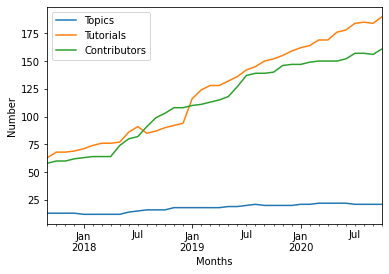
\includegraphics[width=\textwidth]{images/training-material-evolutions.png}
    \caption{Evolution of number of topics, tutorials and contributors over the months}
         \label{fig:material-evolution}
    \end{subfigure}
    \hfill
    \begin{subfigure}[b]{0.5\textwidth}
         \centering
         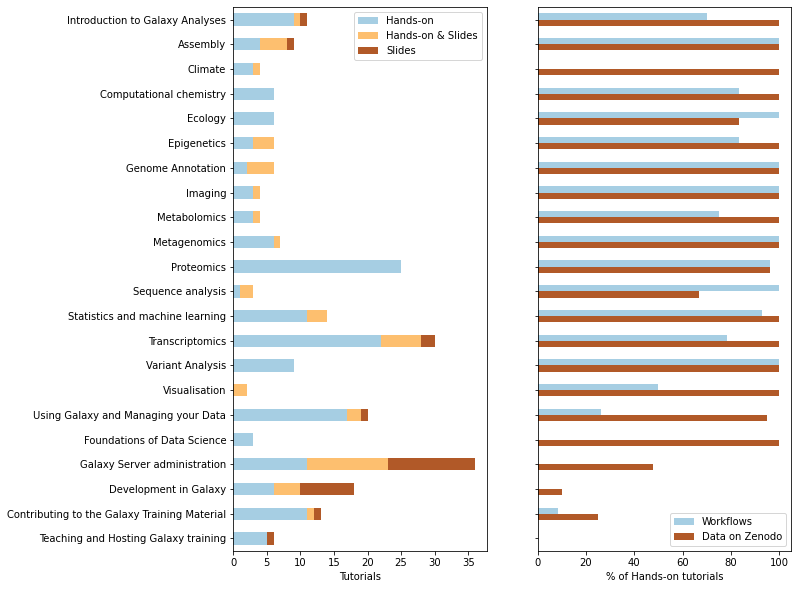
\includegraphics[width=\textwidth]{images/training-material-number.png}
         \caption{Tutorials by topics on the 7th October 2021}
         \label{fig:material-number}
    \end{subfigure}
	\caption{Numbers of tutorials, slides, hands-on tutorials and other material per topics available on the Galaxy Training Material. The Jupyter notebook used to create these figures is available on the GitHub repository for this paper (\url{https://github.com/galaxyproject/GTN-community-paper-2020})}
	\label{fig:material}
\end{figure}

\subsubsection*{Tutorial philosophy}

Tutorials are typically constructed around a real-world \emph{research story}, e.g.\ a published journal article describing an analysis workflow or dataset. 
The tutorial starts by introducing the relevant scientific background, and then proceeds to recreate the analysis, providing details on the relevant scientific and computational concepts involved at each step. The tutorials are composed of alternating theory and hands-on sections, interspersed with formative assessment questions and exercises, and may be supported by a set of introductory slides (Figure \ref{fig:tutorial-skeleton}). Our tutorials are self-contained, i.e. everything needed to complete the tutorials is available from the tutorial page; this includes all the datasets, the workflows, and the list of public Galaxy servers supporting the tutorial. No software installation is needed, and the only technical requirement on the learner is a web browser.


This infrastructure has been developed in accordance with the FAIR (Findable, Accessible, Interoperable, Reusable) principles for training materials \cite{Garcia2020} (Table~\ref{tbl:rulesforfair}). Following these principles enables trainers and trainees to find, reuse, adapt, and improve the available tutorials. 


\subsubsection*{Open, Collaborative, Peer-reviewed tutorials}
To ensure the quality of the tutorials, an open, collaborative, community-driven approach is used as in open-source software. All tutorials are stored in the GitHub repository (\url{https://github.com/galaxyproject/training-material}). Each new tutorial, or update of an existing tutorial, is submitted through a transparent peer-review and curation process. This process relies on editorial teams, i.e. a community of both instructors and/or experts in certain topics, and follows the a similar contribution workflow as other open source projects. Anyone can participate in the review process, but the final decision to approve is made by a maintainer who can accept the content.

\subsubsection*{Community appreciated materials} The materials are not only used during workshops but also by individual learners, as shown by the analytics over the last year. On average, the website is visited 17,000+ times per month (Figure~\ref{fig:analytics-all-users}) with 20\% of returning users, mostly from United States (28.99\% of the visits), India (8.01\%), United Kingdom (6.40\%), Germany (6.20\%) and France (3.90\%).  Since September 2018, over 1,500 individual tutorial feedback forms have been submitted with a high satisfaction rate (more than 85\% had a satisfaction rate of 4 or 5, per Figure~\ref{fig:feedback}).

\subsubsection*{A Vibrant Community}
This project is only as strong as the community behind it and as such we have sought to make it easy to become part of our training community. We provide several avenues for feedback; from the end-of-tutorial feedback form, to a dedicated chat channel on the matrix network (\url{training.galaxyproject.org/chat}) which provides an easy entry point, to callouts on every tutorial welcoming new contributions and guiding would-be contributors through the process, all with the aim to help these new contributors become active members. Every 3 months, community days are organised with community calls, in which we talk together and share news about Galaxy and Training, and a collaboration fest (CoFest), where anyone who would like to contribute, learn how to contribute to the Galaxy Training Material or just catch up with the community is very welcome to join. As a result of this effort, the number of contributors is ever increasing (Figure \ref{fig:material-evolution}) since the beginning of this project.

\subsection*{An Instructor's View: Teaching with Galaxy and its material}

The GTN training materials minimize the amount of time and effort required for instructors to prepare for and run their course or workshop. As an example, we now describe the process used by an instructor who plans to give a workshop on RNA-Seq data analysis to participants who have never used Galaxy or analyzed RNA-Seq data before.

\subsubsection*{Preparing a course or workshop}
During preparation of a workshop, organisers and instructors work together to identify relevant training materials for their event. Our training material is roughly divided into topics such as \emph{Transcriptomics} or \emph{Climate Science} on \url{https://training.galaxyproject.org}. There instructors can find multiple hands-on tutorials - each with different stories - to explain different types of RNA-Seq data analysis. Each tutorial starts with a list of requirements, the expected level of learners, a rough time estimate, questions addressed by the tutorial, as well as learning objectives following Bloom’s taxonomy \cite{Bloom1956} (Figure \ref{fig:tutorial-skeleton}). Each tutorial includes the pre-requisite tutorials and slide decks which are needed to introduce the topic or tutorial, which the instructor can include in their event schedule. By their hands-on nature (Figure \ref{fig:tutorial-skeleton}), the tutorials rely on some predefined data (included in the tutorial metadata), and tools which we analyse in order to list compatible public Galaxy servers.

\subsubsection*{Teaching the workshop}
During the workshop, instructors can introduce the topic using the available slide decks, supported by strong speaker notes. After that introduction, following the tutorial script, the instructor can show in a step-by-step fashion with explanations (boxes) how to interact with Galaxy, upload data, run tools for the analyses, extract workflows, and so on. The tutorial is a fully self-contained teaching resource as described in Figure \ref{fig:tutorial-skeleton}. For first time instructors, The Galaxy Training Network has come together to collect different instructor’s experiences (``Training Philosophies'', \url{https://training.galaxyproject.org/topics/instructors/philosophies/}) and also best practices, providing technical and logistic recommendations, accessible on the website with a series of tutorials (available in ``Teaching and Hosting Galaxy training'' category).

\subsubsection*{Relying on a robust Training Infrastructure}
As \emph{doing} is one of the most efficient ways of learning [\textbf{TODO, CITATION NEEDED}], the instructor encourages participants to do the same as them, either in the same time or later, by providing them access to a Galaxy server and data. There are two main problems in workshop organising: identifying affordable and reliable infrastructure, and locating or developing training materials. The problems share significant commonalities but require very orthogonal skills.
Training materials development requires good pedagogical and writing skills, depth of knowledge about the biological topic, and foresight to plan for student questions or potential errors. Training infrastructure development requires good system administration skills, depth of knowledge about the environment (often Linux), and the foresight to plan for required capacity and scaling.

The needs of training infrastructure are significantly different from normal Galaxy usage. In normal usage, users run workflows or ad hoc analyses, but can accept 30 minute delays in their jobs being processed. A server used in training must process within 5-15 minutes or the course will be impractical to run. 
The provided, small (sub-sampled) training datasets help to achieve this goal, but alone are not enough. The GTN has developed several different approaches which all work in concert to provide re-usable solutions to these problems for the instructor, removing the need for them to either manage the system themselves, or convince their local sysadmin to quickly develop the necessary Galaxy knowledge.

\paragraph*{Training Infrastructure as a Service (TIaaS)}
Many trainers privately raised the issue of the difficulty of locating training infrastructure and Galaxy Europe developed Training Infrastructure as a Service (TIaaS) \cite{Rasche2020} as a response. There they offer ``Galaxy as a service'', sending training jobs to a special queue to run faster ensuring courses run smoothly and efficiently. Following an instructor request for infrastructure, when the workshop begins participants self-register in the course using a keyword provided to them by the instructor. The instructor can then monitor the completion progress of participants without moving around the classroom, and move forward with training more efficiently. TIaaS has proven to be an excellent solution to the training infrastructure problem (Figure~\ref{fig:tiaas}) as trainers can obtain all of the benefits of a large, managed service such as scalability and on-call support. The centralisation of administration means less duplication and waste, and it has been shown to scale well whilst not exerting undue pressure on administrators of existing Galaxy servers. To date TIaaS has been widely used: $>8000$ students taught over 229 events between 2018-06-20 and 2021-11-29, with 64\% using the GTN materials. \textbf{TODO: Update numbers + Include AU, there's another TWO THOUSAND students there.}


\paragraph*{Workflow Testing}
Automated workflow testing provides reassurances to instructors, letting them know that a given tutorial will certainly work on their selected server.
In the GTN framework, Galaxy workflows are developed in parallel with tutorials. The European Galaxy Team created a automated workflow testing project (\url{https://github.com/usegalaxy-eu/workflow-testing/}) to take these workflows, write test cases for them, and then run them every month against a few servers before recording the results. Automated workflow testing provides reassurances that everything is functional in advance of a big workshop. It helps the community of instructors, contributors, and tool users to work in concert to ensure training materials are known to be working.

\paragraph*{Training Data Libraries}

To run the tutorial, the instructor starts by uploading some datasets, stored on Zenodo, into Galaxy. It requires quite some network transfer if 50 students download the same file and load it into Galaxy 50 times in the same time. To limit that, training data can be pre-loaded into a data library and stored as a single copy exists on that server that can be reused as often as needed without incurring additional storage costs.

To make all of the datasets referenced in the GTN framework available in data libraries, the UseGalaxy.* initiative built a service (\url{https://github.com/usegalaxy-eu/shared-data}) which shares these datasets across data libraries of an array of Galaxy servers. While the service was initially constructed for the use of the UseGalaxy.* project, it is open for anyone to join, allowing their administrators to have all of the necessary datasets for training pre-loaded into their servers, without any administration overhead.

\paragraph*{Scaling Training}
Touched upon in the discussion of TIaaS is the problem of scaling, but this problem occurs in two directions: how to scale the students, and how to scale the infrastructure.
Classroom sizes are usually limited by the number of interested participants in the locale, as well as by the availability of suitable venues.
Infrastructure is similarly limited, but with hidden requirements. Running through a tutorial by yourself may execute quickly and look like everything will run smoothly, but some tools have non-obvious memory or CPU requirements that may balloon when giving training for 30 or 100 students.
Both of these issues require planning and some creativity to solve.
TIaaS works to provide scalable infrastructure, the setup underlying the UseGalaxy.eu service allows for the addition of compute resources as needed.
While capacity is available from them, if training needs extend beyond what is possible on their infrastructure, there is the chance to build a cluster on compute resources that a trainer has available (e.g.\ in AWS) and attach these to the UseGalaxy.eu server, providing for essentially infinite scalability of training infrastructure, limited only by the training budget.

\paragraph*{Training with limited Internet access}
Improved internet access also makes the TIaaS offering from Galaxy Europe an increasingly valuable tool for work in LMICs.
Bandwidth limitations and low reliability means that even if internet access has improved markedly it is often not sufficient for bioinformatics work.
Using a Galaxy server located in a region with high quality Internet bypasses these issues as demanding uploads and downloads are kept between the Galaxy server and the external data resources while the process is controlled from a remote location with more limited internet. %(\url{https://galaxyproject.eu/posts/2017/12/10/b3africa/}, \url{https://galaxyproject.eu/posts/2019/11/02/tomas-klingstroem-training-update/}).
Training researchers to train themselves using the Galaxy Training Network materials thereby means that following a basic training session researchers can continue their training through self-studies and also obtain help not only by their personal contacts but also by the wider Galaxy community.

When high quality internet access is not available, the GTN has produced Docker images, allowing offline training, independent from public Galaxy instances.
Every topic has its own Docker image available on Quay.io:  bare-bones Galaxy base image decorated with the necessary tools, workflows, tours and optional data-libraries to follow the tutorials.
Tools are installed based on the workflow files in the tutorials, guaranteeing that the Galaxy container will contain the correct tools and dependencies.
The shared data libraries can be included in the Docker image, or automatically downloaded at the container run, reducing image size.
This provides an ideal training environment where internet access is restricted but data is available, including many LMICs.

\subsubsection*{Instructor Feedback}

In January 2020, we conducted a survey asking how trainers used the available training material. We received answers from 33 trainers, 88\% of which had conducted a training event in the last 3 years.
This sample consisted of a continuum of trainers, from occasional to seasoned trainers. 24\% of trainers gave a training session once in the past 3 years, and 34\% gave 10 or more training sessions, with 10\% more than 25.
Concerning the use of training materials, 79\% of them used GTN resources, and some even developed new GTN materials for the occasion. 
The participating instructors gave 4 or 5 star ratings (within a 1 to 5 scale) to the GTN tutorials, with 91\% of respondents indicating they would absolutely recommend them, confirming the satisfaction scores in the embedded feedback form (Figure~\ref{fig:feedback}).

In addition to the training material, trainers sometimes use resources for enrollment forms and certifications, or add exercises.
Trainers report the need of a few weeks to prepare new material.
This time is reduced to a couple of days when the material already exists in the GTN.
They appreciate that the GTN material is “up-to-date”, stable, and that the community provides a wide variety of analysis relevant to current research.
The trainings are “easy to follow”, have a “great pedagogy” and allow trainees to be “involved in learning”.
The use of GTN material allows them to have more time to focus on the fundamental principles of  analyses and the specific needs of the trainees.

The surveyed trainers all gave training on -omics analyses.
These trainer profiles could evolve with the introduction of training on diverse fields of expertise. In addition to hands-on and slides material, used by respectively 100\% and 72\% of the surveyed, users took advantages of the GTN materials to populate Galaxy instances with relevant tools and/or data (29\% and 38\% respectively).
Some trainers also made use of the extra material on teaching and workshop hosting (24\%) or on training philosophies (10\%) to inform and improve their training events.
The main Galaxy platforms used during these events were Galaxy Europe, Galaxy  Australia, and temporary cloud servers. Trainers also used local Galaxy instances (from their country) and  private servers (from their institution).
59\% of them relied on TIaaS (Training Infrastructure as a Service). Its usage was highly rated (100\% 5 stars) and highly recommended (94\% 5 stars).

69\% of the surveyed trainers are contributors to the training material, and among those who are not, 55\% declare planning to become one in the future.

\subsection*{A Contributor's View: developing GTN tutorials}

The GTN framwework is inherently collaborative and community-driven, and comprises a growing number of contributors (Figure~\ref{fig:material-number})  with expertise in a wide range of scientific and technical domains. Given this highly collaborative nature of a community with very different skill sets, the GTN framework has evolved over the years to facilitate the contribution and maintenance of the tutorials. We aim to adhere to best-practice guidelines for collaborative lesson development described in \cite{Devenyi_2018} (Table~\ref{tbl:tensimplerules}). The structure of the tutorials and repository has been made modular with unified syntax and use of snippets enabling easy access for authors to add common tips and tricks new users might need to know. This system allows for easy updating of all tutorials, if there is a change in tools or interface. More generally, we continually strive to lower contribution barriers for content creators by providing a framework that is easy to use for training developers regardless of their level of knowledge of the underlying technical framework.

The GTN framework ensures easy contribution and maintenance, through a diverse set of tools and standards. 
This section describes the typical process a tutorial contributor will go through when developing a new tutorial (Figure \ref{fig:contributing}).

\begin{figure}[!ht]
	\centering
	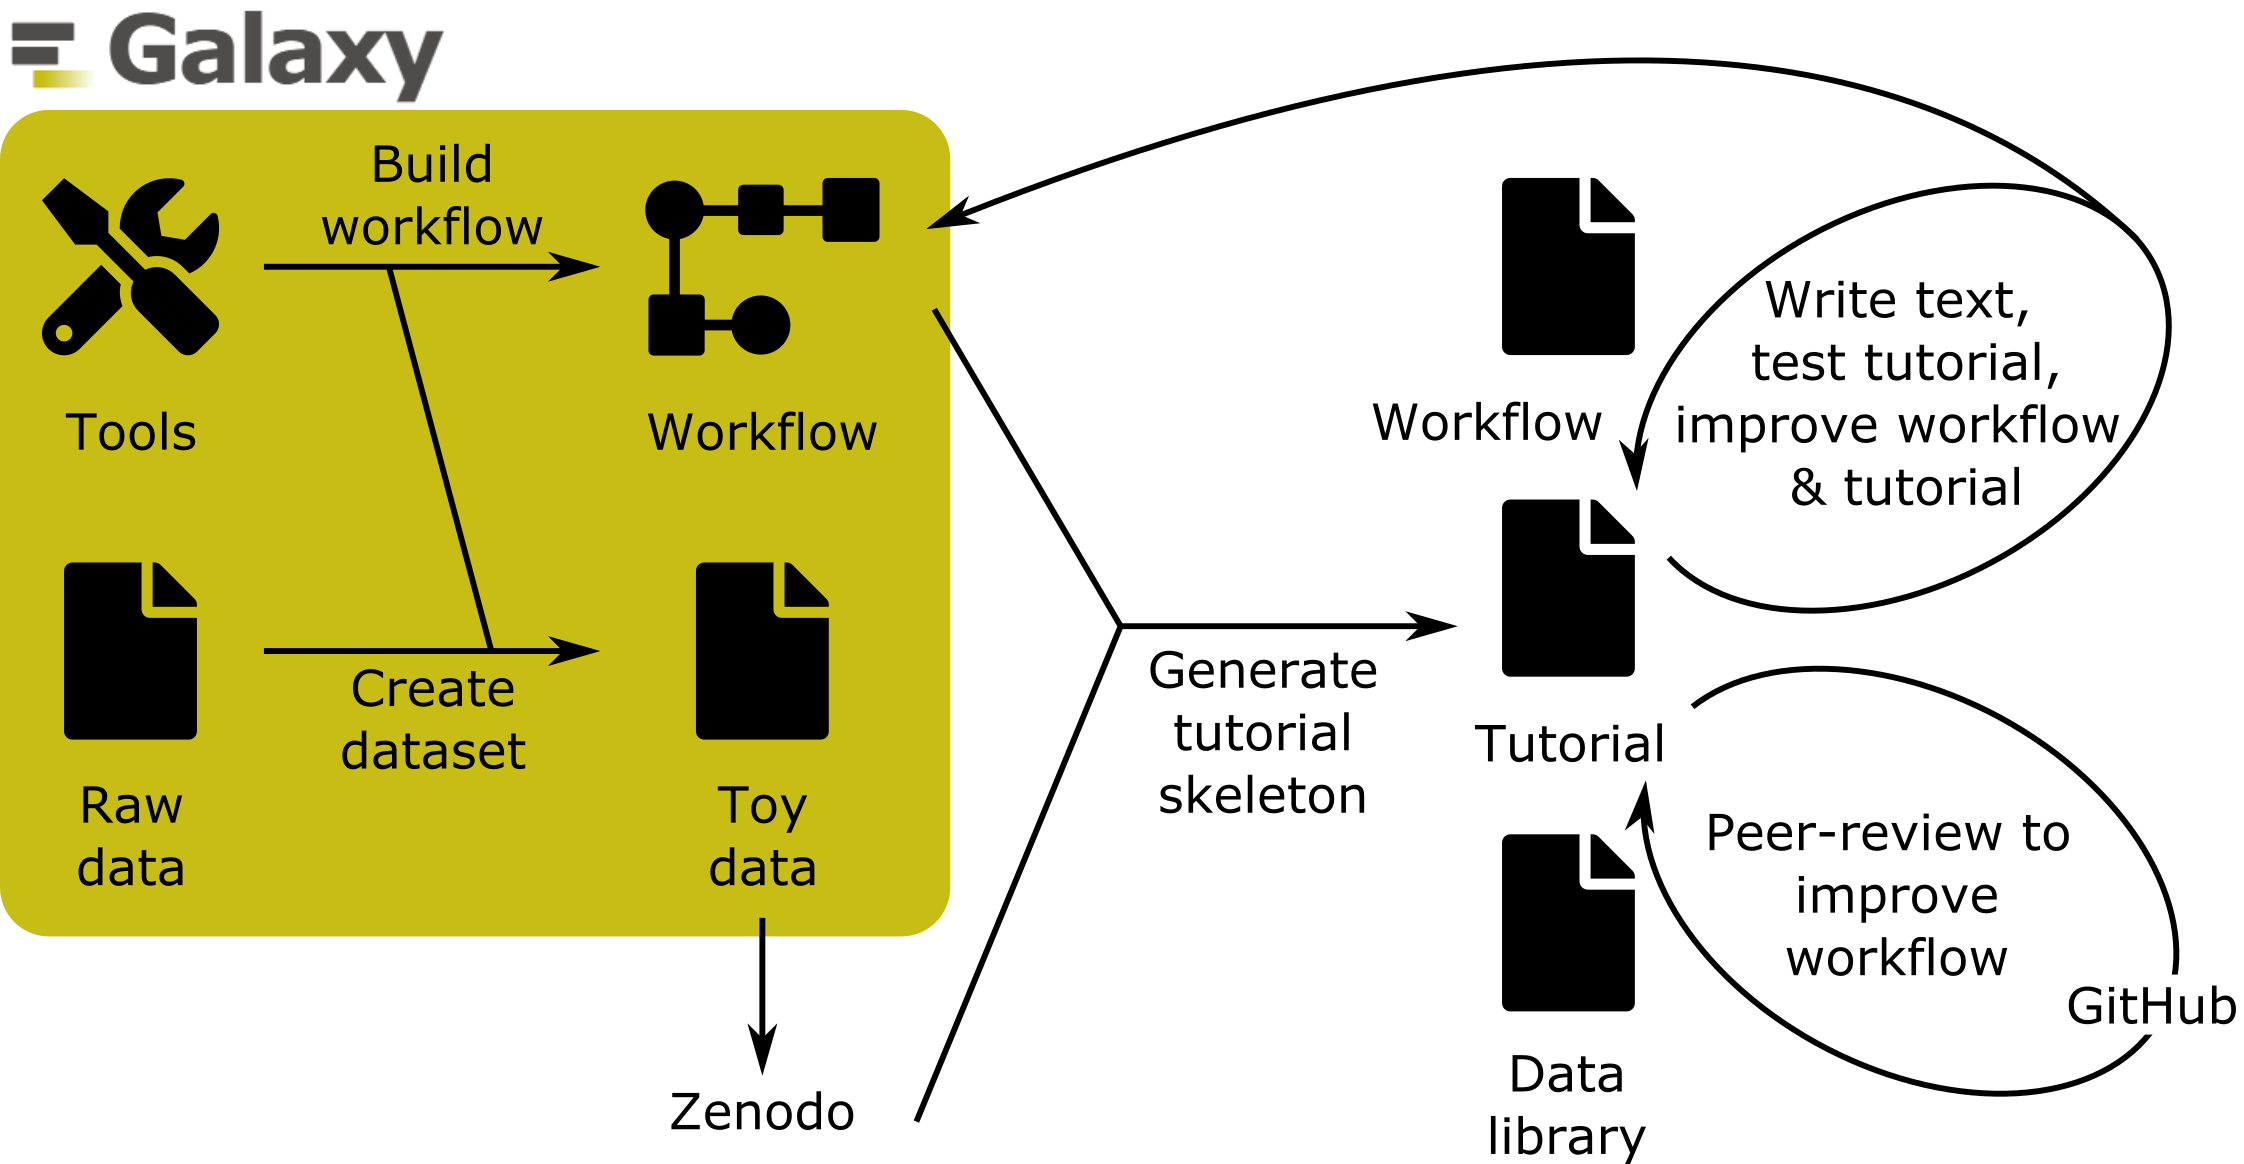
\includegraphics[width=\textwidth]{images/contributing.png}
	\caption{Typical process to create a new tutorial\label{fig:contributing}}
\end{figure}

\subsubsection*{Contributing Tutorials}

To get acquainted with the tutorial development methodology, the contributor starts by consulting a set of dedicated tutorials in the \emph{Contributing} topic. These tutorials provide a step-by-step guide to creating a tutorial in the GTN framework. These tutorials range from technical guides concerning the format (tutorials and slides written in Markdown) and website generation (with Jekyll), to pedagogical best practices and submission of changes to GitHub. These tutorials help create a first example tutorial. After completing the tutorials, the contributor can move on to writing their own tutorial.

\subsubsection*{Building workflow and identifying data}

The tutorials try to follow the “learn by doing” approach by combining both theoretical and practical sections. The practical sections (or hands-on) are supposed to be done by running tools on Galaxy. When developing a tutorial, contributors usually follow a known pipeline. So the first step is to build a workflow in Galaxy with the needed tools in the correct order. This workflow then helps to build the tutorial, and it usually evolves with the writing of the tutorial.

After building the workflow, the first task is to select some data to use for the practical sections. The selected data must be informative enough to illustrate the meaning of using a tool or a given technique, but not too big to require long waiting times for processing during a workshop. Upload and download of files into and out of Galaxy is usually quick, but the time taken for a tool to run can be long. Tool run times of no more than 10-15 minutes are recommended. Typically, the selected data could be a toy dataset created from scratch or even better the informative subset of a full real-life dataset. For example, in the ATAC-seq tutorial, to build a toy dataset with meaningful reads, the authors ran the workflow until the mapping step on the original FastQ file and extracted read IDs which map on the smallest chromosome. In order to keep enough diversity in the toy dataset, they also randomly extracted the IDs of 1\% of the reads from the original dataset. They concatenated both lists of IDs and extracted the corresponding reads in the original FastQ files.

\subsubsection*{Planemo Training Development Kit}

To re-create the analyses in a tutorial, hands-on sections (Figure \ref{fig:tutorial-skeleton}) provide details about the tools to run and the parameters. Creating and formatting these sections can be cumbersome. To simplify the process, we have created a \emph{Tutorial Development Kit} within the Planemo tool, a command-line utility to assist in developing Galaxy artifacts. This allows contributors to generate a tutorial skeleton from a Galaxy workflow as a starting point for tutorial creation.
This skeleton contains the metadata section, auto-generated hands-on boxes for every tool, template question boxes, and instructions for the tutorial creators about how to proceed. 
This process greatly reduces the development time, and allows tutorial creators to focus on the scientific content of the tutorial, rather than the technical implementation details of the framework.

In order to further lower the contribution barrier, this \emph{Planemo Tutorial Development Kit} has been encapsulated into a webservice (\url{https://ptdk.herokuapp.com/}) wherein training material authors can point to a public workflow on one of the UseGalaxy.* servers, and generate the tutorial skeleton automatically.
This removes the need for contributors to install and run the tool locally.
 We have found that this approach saves time for not only the contributors but also the reviewers as the training materials contributed using this method adhere well to the training material’s style guide.

%\begin{figure}[!ht]
%	\centering
%	\includegraphics[width=0.8\textwidth]{images/tool-in-tutorial.png}
%	\caption{An automatically generated hands-on box using the Planemo Training Development Kit. This box corresponds to the running of a single tool. All of the relevant parameters have been automatically extracted from the workflow definition file used to generate the skeleton. Where parameters are left to their default values, they are not listed in this box, but where they must be changed from their default values, detailed hands-on instructions are provided.\label{fig:planemo}}
%\end{figure}
%% BB: update image as Rename step is not there in generated hands-on

The Training development kit also offers commands to generate the auxiliary tutorial files, such as the \verb+data_library.yaml+ file.
This file describes the required input datasets. All datasets used in tutorials are stored on Zenodo and associated with a Digital Object Identifier (DOI) making them citable and discoverable.
This Zenodo DOI can be provided as a parameter to the \emph{Planemo Tutorial Development Kit}, to autogenerate the data library configuration file.
This files makes it easy to populate a \emph{Shared Data Library} on a Galaxy server using the Ephemeris tool (\url{https://ephemeris.readthedocs.io}), which will greatly speed up the process of configuring a Galaxy server to support the tutorial.

To develop their new tutorial, the contributor creates a Galaxy workflow in one of the UseGalaxy.* servers, makes it public, and uploads the input data on Zenodo to get a DOI. They provide this information together with tutorial title and topic to the \emph{Tutorial Development Kit} web-server. They obtain an archive including a folder with the tutorial skeleton, the workflow, and the data library configuration file. In this skeleton, the contributor fills in the metadata, adds the scientific background and story between the hands-on boxes, and adds some formative assessment questions and answers.

\subsubsection*{Modularity}

To avoid duplication of content between tutorials, we have developed a set of modular tutorial components, called \emph{snippets}, which can be easily re-used across tutorials.
For example, common tasks in Galaxy such as starting a workflow or creating a new history, will be steps in the majority of tutorials. In order to avoid duplication, and making it easier to apply updates to these common steps when the Galaxy interface changes, we have modularized these sections. The contributor can include these snippets at any place in a tutorial with a single import instruction. 
This again allows them to focus on the scientific topic at hand, rather than the Galaxy interface steps.
%% animated GIF associated with snippets

\subsubsection*{Local Preview and Testing}

During tutorial development, contributors want to preview how their tutorial will look online.
To this end, we have provided simple functions to generate a local preview of the entire website with a single command. Whenever the tutorial files are updated, the preview will be regenerated as well.
In addition to a visual inspection of the generated web pages, our framework offers a suite of testing tools, allowing contributors to check that their tutorial meets the guidelines.
These tests include checks of whether all required metadata is present and in the correct format, whether any links within the tutorial are valid, and whether files are correctly formatted.
This will help contributors and reviewers to quickly identify potential problems with a tutorial.

\subsubsection*{Peer Review}

Once a contributor is happy with their tutorial, they can create a \emph{pull request} (PR) to the GTN GitHub repository where all tutorials are kept.  (\url{https://github.com/galaxyproject/training-material}).
The contribution will then undergo a peer-review process.
This process is open to any volunteers from the community; they will check the tutorial, both in terms of formatting and scientific content.
These reviewers can make suggestions for updates, and start a discussion with the tutorial contributor(s).
Typically there will be two or three reviewers for any given pull requests.
Based on this feedback the contributor(s) will update the tutorial, and this cycle of update and review will continue until both contributor(s) and reviewers are happy with the training materials.
In order to aid the reviewers, all available tests in our framework are automatically run on incoming pull requests, using the GitHub Actions framework.
These tests aid in the identification of any errors in the tutorial, and prevent non-compliant tutorials from being merged.

Community is how the GTN survives and thrives: instead of having a central authority for approving new training content or changes, we delegate the final decisions about the contributions to a set of responsible persons.
For each topic within the training materials, the GTN has encouraged several prominent community members who are regular contributors to step up as topic maintainers, i.e. people who feel responsible for content in that domain and are empowered to review, approve, and merge content in that topic.
Topic maintainers are not the only group encouraged to review new pull requests and content, anyone from inside and outside of the community is welcome and encouraged to review new training materials.
While non-maintainers cannot merge changes, their review contributions are an important part of this project.
Reviews are the cornerstone of this project as shown by our very active reviewers in Figure~\ref{TODO}

\subsubsection*{Tutorial maintenance and feedback}

Tutorials are dynamic entities; underlying analysis tools receive updates, new tools are developed, and the Galaxy interface itself changes regularly.
As a result, tutorials must undergo regular updates as well to reflect the state-of-the-art in the scientific domain, and correctly reflect the latest available version of the tools and the Galaxy interface.

Instructors preparing for their next workshop often check the tutorials as preparation, and in the process identify the places where the tutorial should be updated.
If the instructors feel comfortable making these changes themselves, they can open a pull request proposing the changes.
If not, they can create an \emph{issue} on GitHub to request the changes.

Furthermore, learner feedback is one of the most valuable resources to inform training improvements.
Anybody using the tutorials will find a feedback form at the end of it, where they can indicate any mistakes in the tutorial, or make suggestions for more general improvements. Many of the updates to the GTN framework have come from suggestion by learners in workshops.
As an example, during one workshop a participant complained of the trouble copying lists of URLs or other code blocks easily; as a result we realised we could implement a copy button which would automatically copy the text on click, and even implemented the feature before the next day of the course.

Any feedback received is posted publicly on the GTN GitHub repository (unless the user indicated it should remain private), enabling the entire community to view and address the feedback.
This public feedback ensures a short feedback loop between content consumers and the tutorial authors, and keeps the authors accountable for their content, as seen in our user reviews (Figure~\ref{fig:feedback}).

This open strategy for content creation and updates is paying off.
Since the beginning of the project in the middle of 2016, over 1,500 pull requests have been created to add or update tutorials (Table~\ref{tbl:pullRequestReviewing}).

\begin{table}[]
\begin{adjustwidth}{-2.25in}{0in} % Comment out/remove adjustwidth environment if table fits in text column.
	\centering
	\caption{Statistics about Pull Request on GitHub repository since 2016.\label{tbl:pullRequestReviewing}}
	\begin{tabular}{l|p{0.2\textwidth}p{0.2\textwidth}p{0.2\textwidth}p{0.2\textwidth}}
 & Number & Reviews and comments (mean number per PR) & Reviewers (mean number per PR) & Duration (mean per PR) \\\hline
Pull Requests to add tutorial(s)  & 253  & 10.8  & 2.8 & 31 days\\
Pull Requests to update tutorial(s) & 1,286 & 3.3 & 1.7 & 9 days\\
Other Pull Requests & 599 & 2.4 & 1.5 & 5 days\\
	\end{tabular}
\end{adjustwidth}
\end{table}

Thanks to a fast turnaround (on average, it takes \~20 days between the opening of a pull request and its merge), tutorials are regularly updated and iteratively improved over time, keeping the material relevant and of a high quality.
Indeed, each tutorial undergoes (on average) a pull request every month to update it. Some highly used tutorials, like the “Reference-based RNA-seq” tutorial, got alo 50 pull requests over the last 3 years, on average one every 3 weeks.

\subsubsection*{Community Support}

If contributors encounter difficulties in any part of their contribution process, or simply want to discuss some aspects of their tutorials, they can seek help on the GTN chat (\url{training.galaxyproject.org/chat}). This channel is always active due to the large community covering many time zones.
Additionally, they may participate in our quarterly online contribution fests designed to support contributors and collaborate on tutorial updates and additions.

The Galaxy Training Network community has grown significantly since its inception (Figure~\ref{fig:material-evolution}).
Within two years after the start of the project, we had 77 members who wanted to be recognised as contributors to the training materials.
In the past two years, we have doubled again to 150 recognised contributors.
All of these contributors are publicly recognised in our \emph{“Hall of Fame”} (\url{https://training.galaxyproject.org/training-material/hall-of-fame/}).
Notably, these are the subset of contributors who wanted to be recognised; numerous others have contributed small fixes and one-off corrections where they did not choose to self-identify as one of the contributors.

\section*{Conclusion}

From the start of the Galaxy project, education has been an important focus. Offering training as part of conferences or in the form of dedicated workshops has helped to grow and foster the worldwide Galaxy community and has brought (biological) data analysis to a broad audience. Much training material has been collected and made available on the Galaxy project website. In its original form, the collection lacked a proper structure, and most of those ad-hoc assembled materials became out-of-date soon after publication.

The Galaxy Training Network has created the Galaxy Training Platform. It is maintained in GitHub and has made it possible to coordinate and structure all those previous efforts in a sustainable way. It makes it easy to manage the addition of new tutorials and/or updating existing ones. Additionally, efforts have been directed to build a powerful training infrastructure while keeping contribution barriers as low as possible. Thus, it has become a valuable resource for the trainees, the instructors and the developers of training content.

Given the feedback from learners, instructors and contributors, new features are currently in development. We are extending efforts to integrate videos to support the slides, but also videos to show some specific aspects of Galaxy interface. To avoid the cumbersome aspect of the updating these videos, we are developing a framework to generate and update them automatically.
In the instructor survey, the trainers have been asked about the improvement they wished to see in the GTN resources. One of the concerns is the access to computational resources, such as using public instances, or having backup servers if the server dedicated to the workshop encounters a problem.
Another important need is the access to GTN material metadata, such as: what new version of training has been published, what new training subject could require contributors. Users suggest that the pedagogic value of training materials could be improved by directing the users to different training depending on their level of expertise, and to provide more context to the analyses.
Some trainers would like more interactivity with the tutorials through exercises or through facilitating the parallel between the tutorial and the Galaxy instance. We plan to answer these suggestions by implementing them. 
To support the instructors and build a community of instructors, we are also implementing with the Gallantries project and in collaboration with ELIXIR, a Train the Trainer program and a mentoring program for instructors. For contributors, we are also working with editors to implement a system for publication of each tutorial via article with limited extra work.

The Galaxy Training Network aims to continue its effort in developing and maintaining this powerful training framework.

\section*{Supporting information}

% Include only the SI item label in the paragraph heading. Use the \nameref{label} command to cite SI items in the text.
%\paragraph*{S1 Table.}
%{\bf Bold the title sentence.} Add descriptive text after the title of the item (optional).

\clearpage
\paragraph{S1 Figure: Graph of Contributions over Time}
\begin{figure}[!ht]
	\centering
	\includegraphics[width=0.8\textwidth]{images/commits.png}
	\caption{Graph of contributions to the training materials repository\label{fig:contributions}}
\end{figure}

\clearpage
\paragraph{S2 Figure: TIaaS dashboard}
\begin{figure}[!ht]
	\centering
	\includegraphics[width=0.8\textwidth]{images/tiaas.png}
	\caption{The dashboard provides anonymised observability into class progress, trainers can see at a glance if everyone has completed the quality control steps, or if there are any errors that they should ask the students to raise with the class.\label{fig:tiaas-dashboard}}
\end{figure}

\clearpage
\paragraph{S3 Table: Ten Simple Rules}
\begin{table}[!ht]
	\centering
	\caption{Implementation of the ``Ten simple rules for collaborative lesson development''\cite{Devenyi_2018} in the training material
    \label{tbl:tensimplerules}}
	\begin{tabular}{p{0.5\textwidth}p{0.5\textwidth}}
		\textbf{Rules}                                      & \textbf{Implementation in the GTN framework} \\
		Clarify audience                                    & Tutorial metadata includes level indicators (introductory, intermediate, advanced) and a list of prerequisite tutorials as recommended prior knowledge. This information is rendered at the top of each tutorial. \\
		Make lessons modular                                & Development of small tutorials linked together via learning paths \\
		Teach best practice lesson development              & A topic \emph{Contributing to the Galaxy Training Material} including 10 tutorials describing how to create new content. Furthermore, quarterly online collaboration fest (CoFests) are organized, where contributors can get direct support. Development of a Train the Trainer program and a mentoring program for instructors, in which lesson development is taught \\
		Encourage and empower contributors                  & Involve them in reviews. Mentor them. Encourage them to become maintainers. \\
		Build community around lessons                      & Quarterly online collaboration fest (CoFests) and Community calls. Chat (Gitter channel) \\
		Publish periodically and recognize contributions    & Author listed on tutorials. Hall of fame listing all contributors. Full tutorial citation at the end of the tutorial. Tweet about new or updated tutorials. List of new or updated tutorials in Galaxy Community newsletter. Soon: publication of tutorials via article \\
		Evaluate lessons at several scales                  & Tutorial change (Pull Request) review. Embedded feedback form in tutorials for trainee feedback. Instructor feedback. Automatic workflow testing \\
		Reduce, re-use, recycle                             & Sharing content between tutorials, specially using snippets. Development of small modular tutorials linked by learning paths \\
		Link to other resources                             & Links to original paper, documentation, external tutorials and other material \\
		You can't please everyone                           & but we can try (several different Galaxy introduction tutorials for different audience). Aim to clearly state what the tutorial does and does not cover, at the start.  \\
	\end{tabular}
\end{table}

\clearpage
\paragraph*{S4 Table: 10 Simple Fair Rules}
\begin{table}[h!]
	\centering
    \caption{Implementation of the ``10 simple rules for making training materials FAIR'' \cite{Garcia2020} in the GTN training material framework
    \label{tbl:rulesforfair}}
	\begin{tabular}{p{0.4\textwidth}p{0.6\textwidth}}
		\textbf{Rules}                                                                & \textbf{Implementation in GTN framework}\\\hline
		Plan to share your training materials online                                  & Online training material portfolio (\url{https://training.galaxyproject.org/}), managed via a public GitHub repository (\url{https://github.com/galaxyproject/training-material})\\
		Improve findability of your training materials by properly describing them    & Rich metadata associated with each tutorial that are visible and accessible via schema.org on each tutorial webpage\\
		Give your training materials a unique identity                                & URL persistency with redirection in case of renaming of tutorials.
		Data used for tutorials stored on Zenodo and associated with a Digital Object Identifiers (DOI) \\
        Register your training materials online                                       & Tutorials automatically registered on TeSS, the ELIXIR's Training e-Support System (\url{https://tess.elixir-europe.org/})  \\
        If appropriate, define access rules for your training materials               &	Online and free to use without registration \\
        Use an interoperable format for your training materials                       &	Content of the tutorials and slides written in Markdown. Metadata associated with tutorials stored in YAML, and workflows in JSON\\
		Make your training materials (re-)usable for trainers                          & Online. Rich metadata associated with each tutorial: title, contributor details, license, description, learning outcomes, audience, requirements, tags/keywords, duration, date of last revision. Strong technical support for each tutorial: workflow, data on Zenodo and also available as data libraries on UseGalaxy.*, tools installable via the Galaxy Tool Shed, list of possible Galaxy instances with the needed tools. (Figure \ref{fig:tutorial-skeleton})\\
		Make your training materials (re-)usable for trainees                          & Online and easy to follow hands-on tutorials. Rich metadata with ``Specific, Measurable, Attainable, Realistic and Time bound'' (SMART) learning outcomes following Bloom's taxonomy. Requirements and follow-up tutorials to build learning path. List of Galaxy instances offering needed tools, data on Zenodo and also available as data libraries on UseGalaxy.*. Support chat embedded in tutorial pages. (Figure \ref{fig:tutorial-skeleton})\\
		Make your training materials contribution friendly and citable                & Open and collaborative infrastructure with contribution guidelines, a CONTRIBUTING file and a chat. Details to cite tutorials and give credit to contributors available at the end of each tutorial (Figure \ref{fig:tutorial-skeleton}).\\
		Keep your training materials up-to-date                                       & Open, collaborative and transparent peer-review and curation process. Short time between updates (Table \ref{tbl:pullRequestReviewing})\\
	\end{tabular}
\end{table}




\paragraph{S5: Analytics}
\begin{figure}[!ht]
    \centering
    \begin{subfigure}[b]{0.45\textwidth}
         \centering
         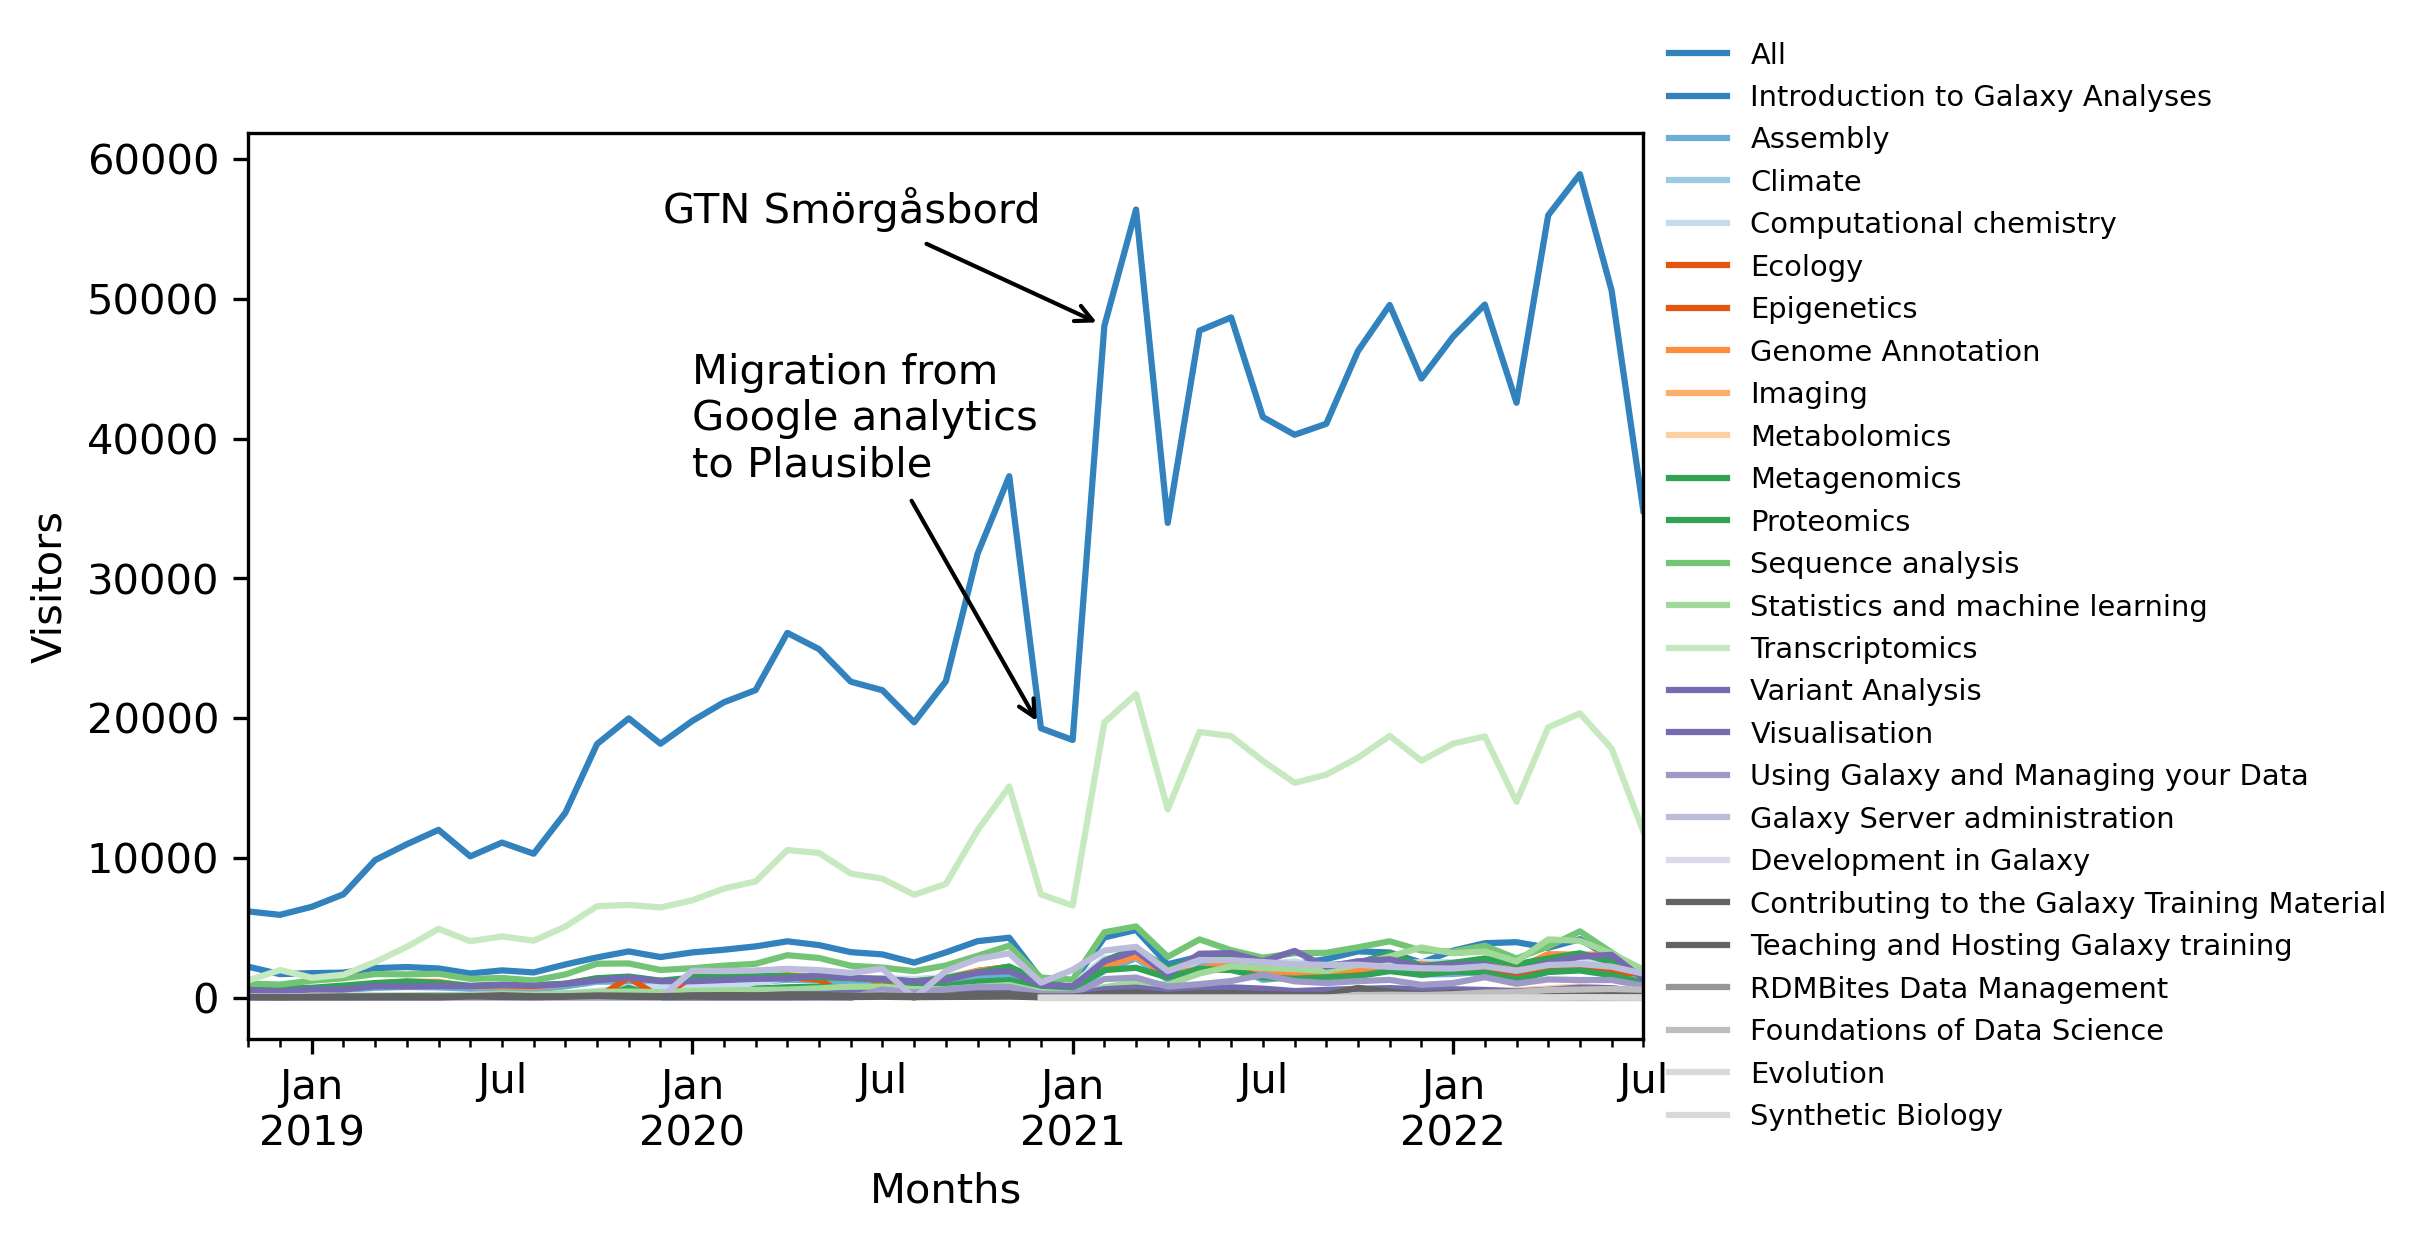
\includegraphics[width=\textwidth]{images/analytics-all-users.png}
         \caption{Number of users per months}
         \label{fig:analytics-all-users}
    \end{subfigure}
    \hfill
    \begin{subfigure}[b]{0.45\textwidth}
         \centering
         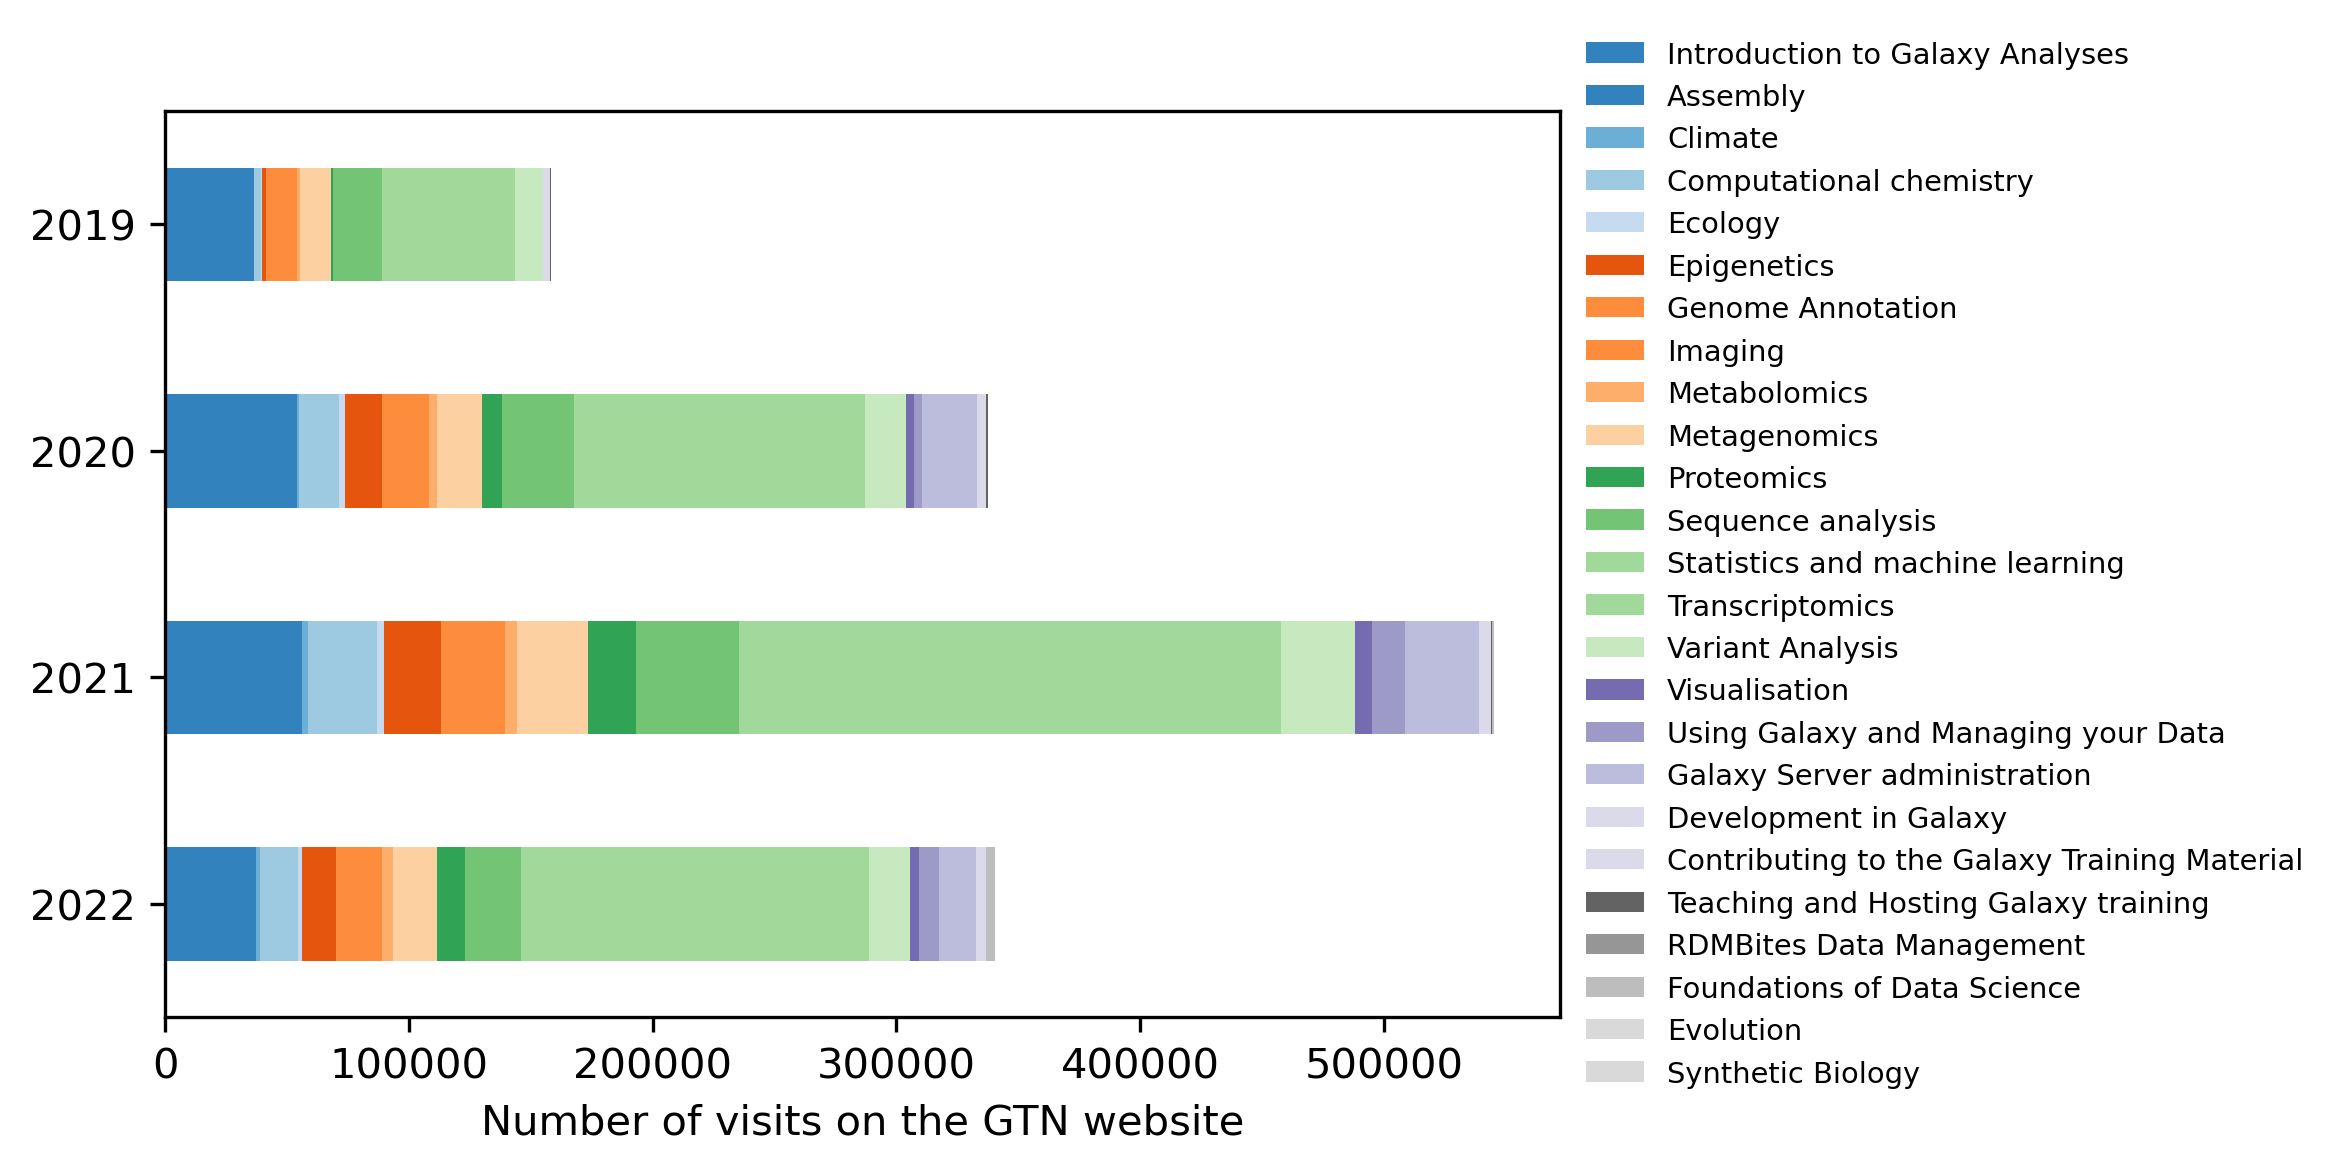
\includegraphics[width=\textwidth]{images/analytics-topics-users.png}
         \caption{Number of users per topics}
         \label{fig:analytics-topics-users}
    \end{subfigure}
	\caption{Number of visits per month on \url{http://training.galaxyproject.org/} given the Google Analytics statistics. The Jupyter notebook used to create these figures is available on the GitHub repository for this paper (\url{https://github.com/galaxyproject/GTN-community-paper-2020}).}
	\label{fig:visits}
\end{figure}

\paragraph{S6: Feedback}
\begin{figure}[!ht]
	\centering
	\begin{subfigure}[b]{0.7\textwidth}
         \centering
         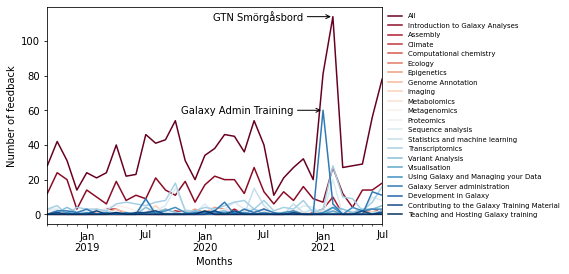
\includegraphics[width=\textwidth]{images/feedback.png}
         \caption{Number of feedback over months}
         \label{fig:feedback-}
    \end{subfigure}
    \hfill
    \begin{subfigure}[b]{0.7\textwidth}
         \centering
         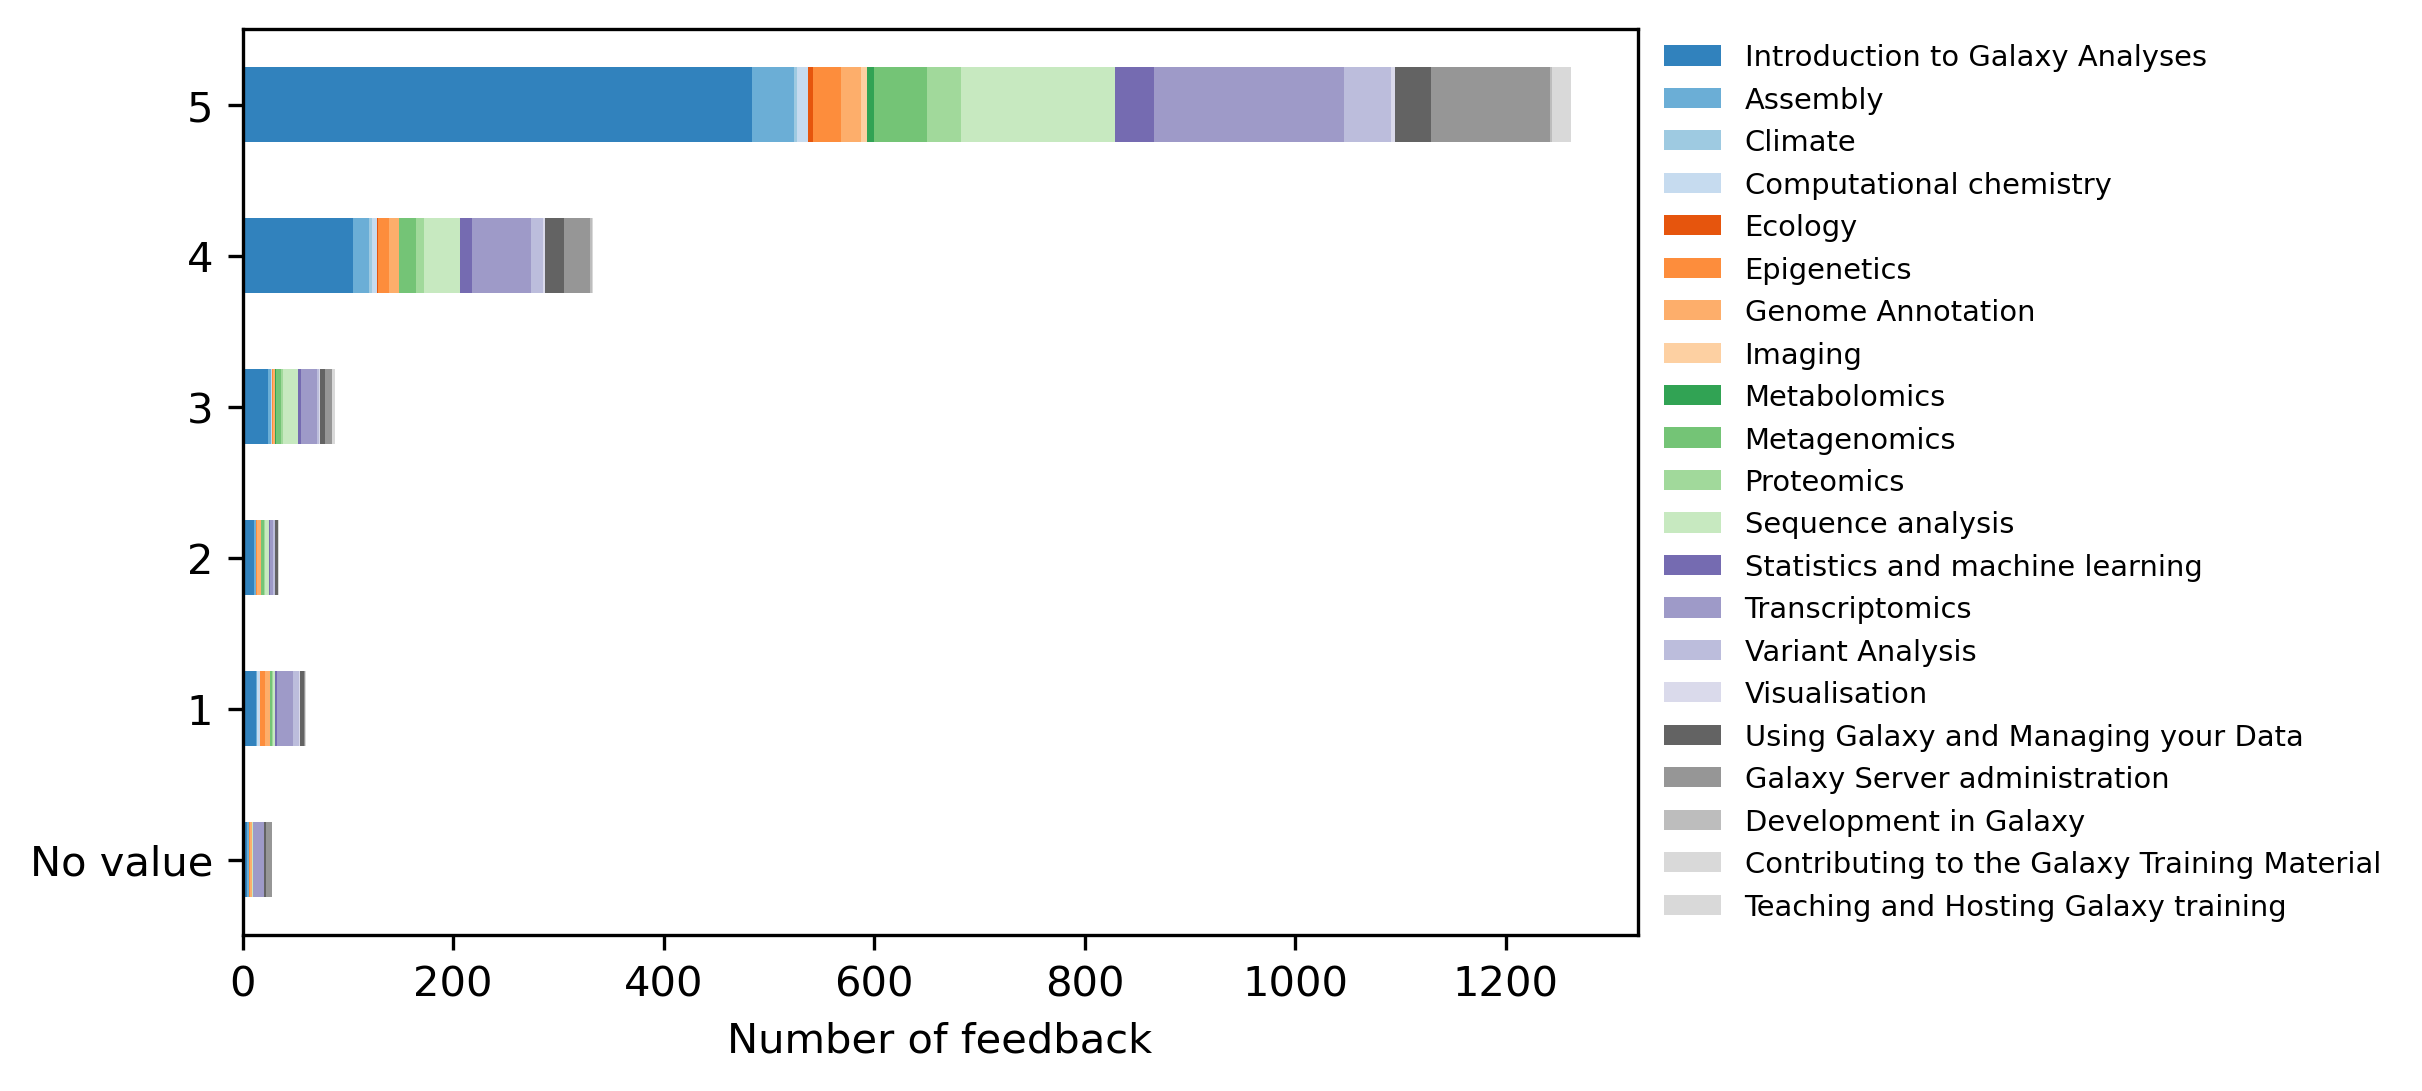
\includegraphics[width=\textwidth]{images/feedback-scores.png}
         \caption{Scores for feedback}
         \label{fig:feedback-scores}
    \end{subfigure}
	\caption{Number and results of the embedded feedback in the tutorials. Three questions are asked in the form: ``How much did you like this tutorial?'' (from 1 (bad) to 5 (great)), ``What did you like?'', ``What could be improved?''. The Jupyter notebook used to create these figures is available on the GitHub repository for this paper (\url{https://github.com/galaxyproject/GTN-community-paper-2020}).
    \label{fig:feedback}}
\end{figure}


\paragraph{S7; Skeleton}
\begin{figure}[!ht]
	\centering
	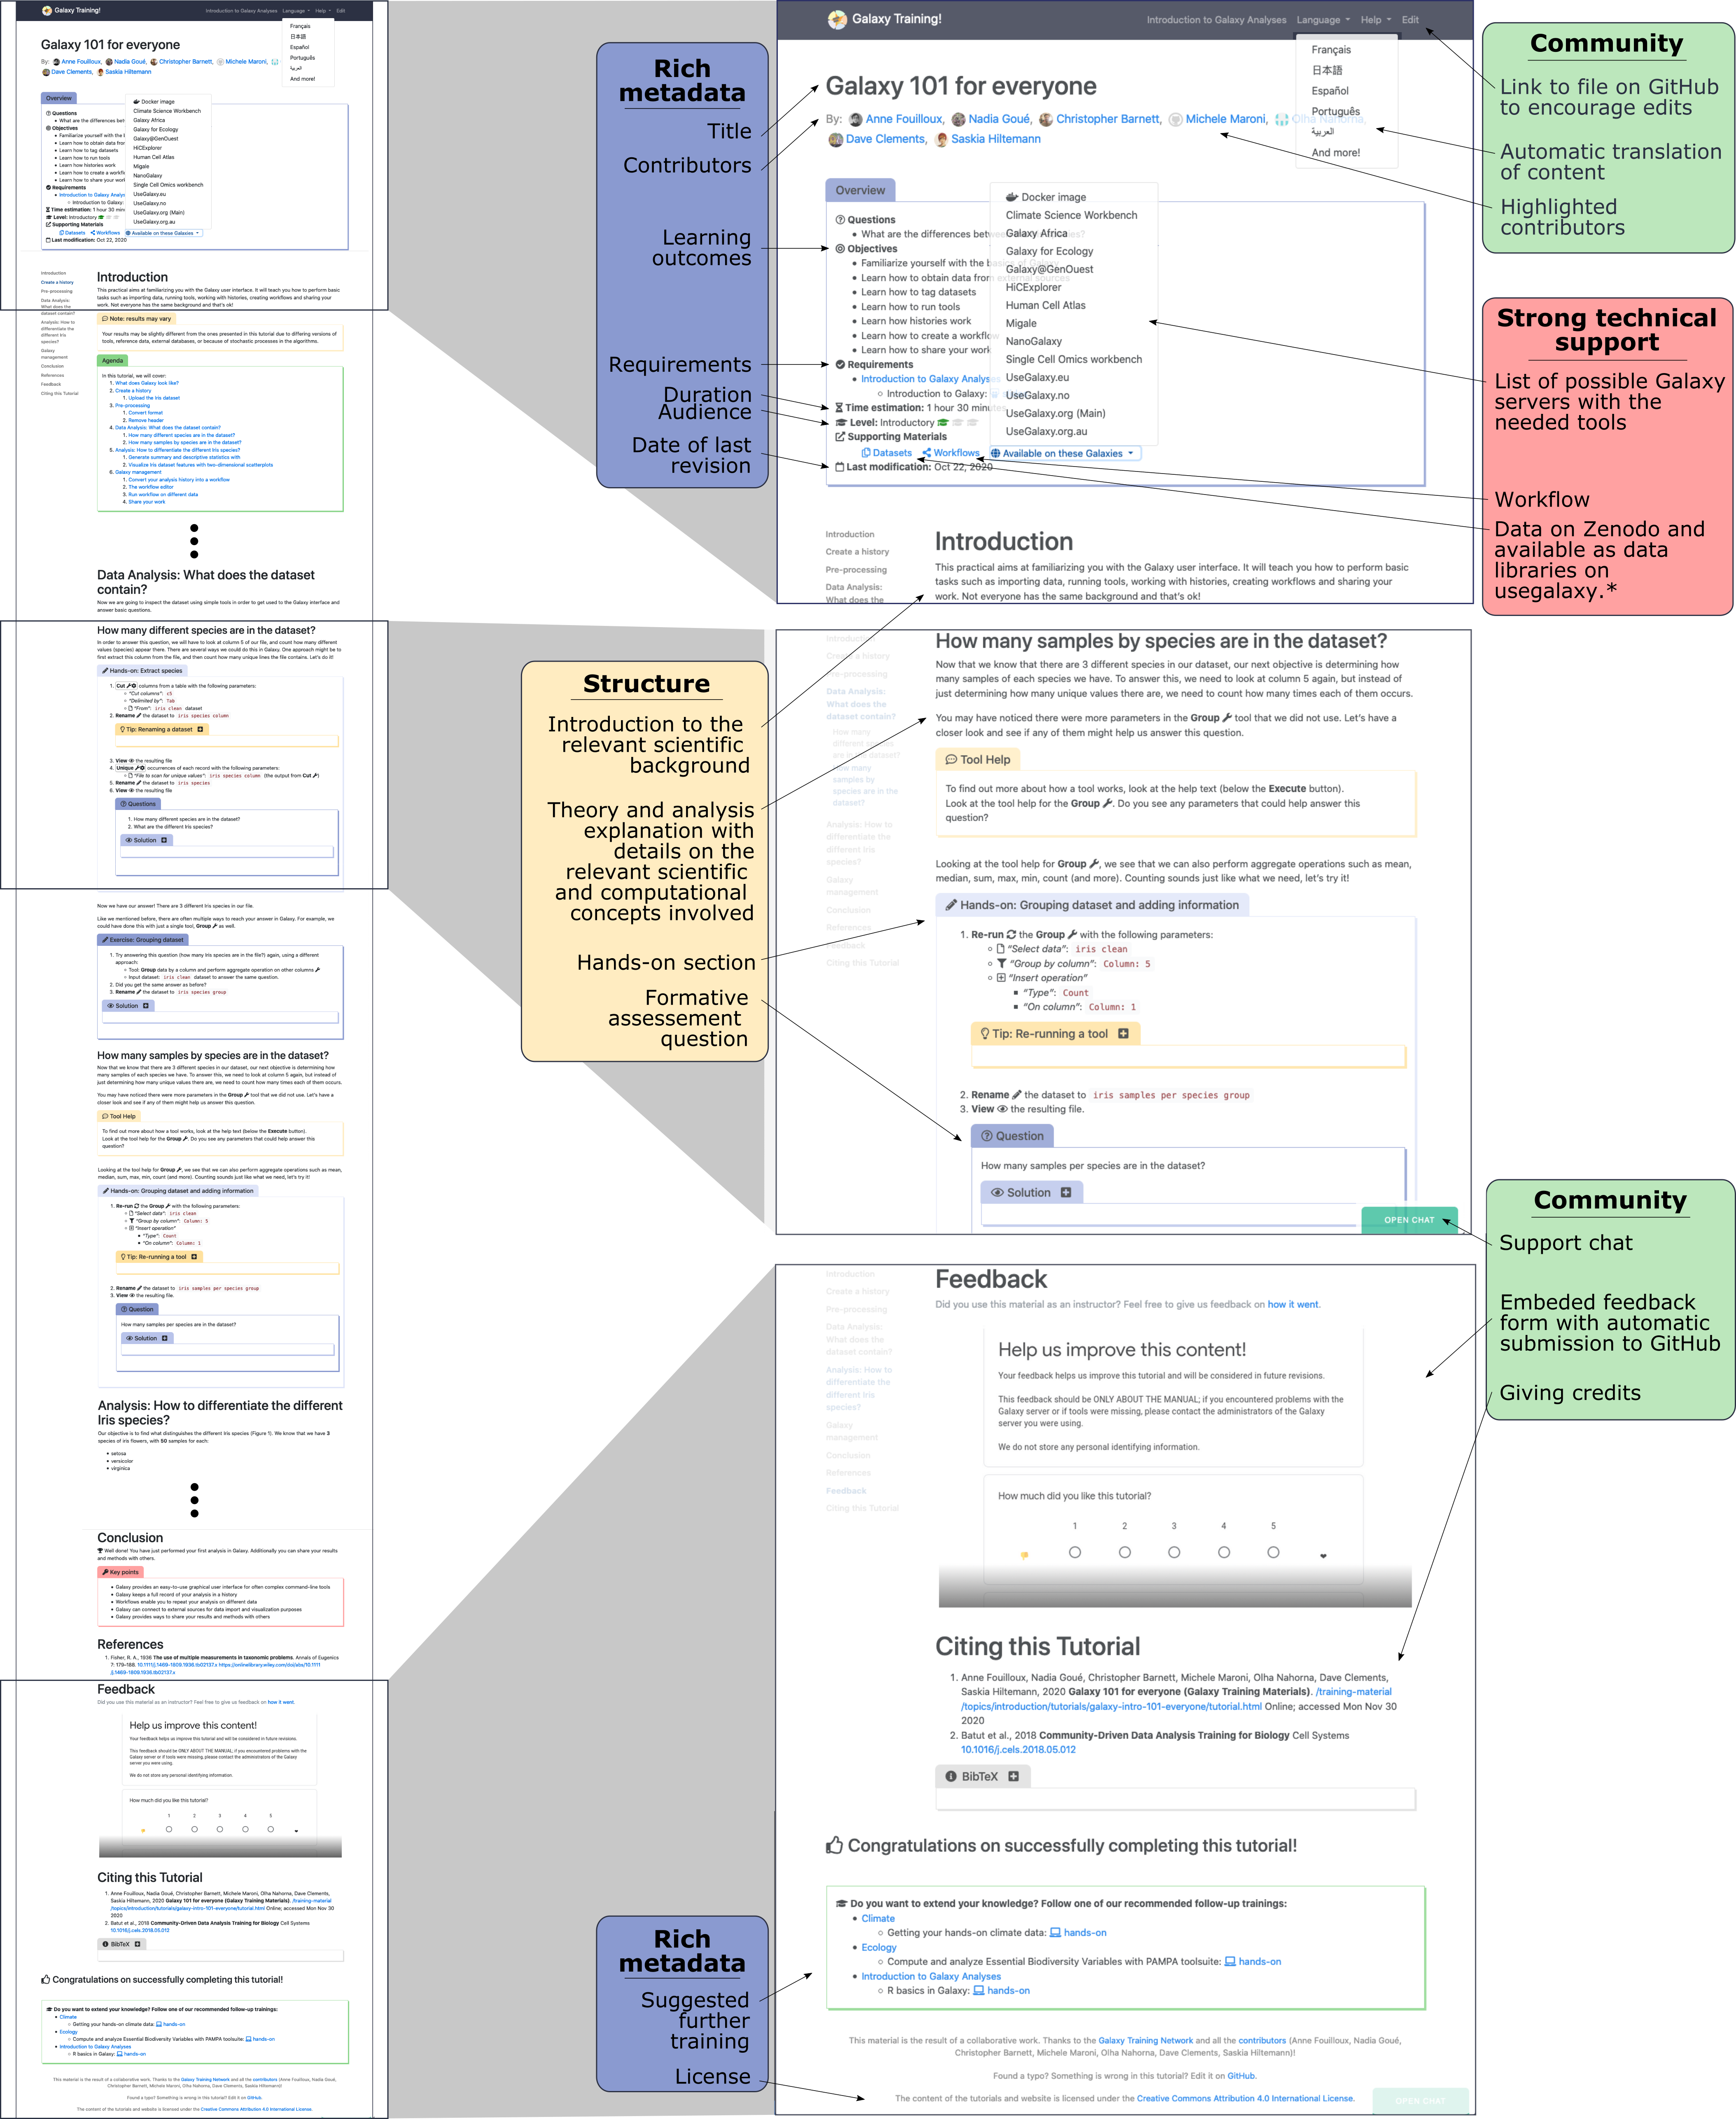
\includegraphics[width=\textwidth]{images/tutorial_skeleton.png}
	\caption{Tutorials are generally quite long and complex documents created from simple plain text documents. They feature a large header box with metadata about the tutorial (audience level, pre-requisites, supporting documents, recent recordings of a live teacher giving this tutorial) which provides strong technical support for teachers and self-studying students. The tutorial content itself is enhanced by a clear hierarchical structure throughout the tutorial and important actions for learners are highlighted with the use of boxes. Hands-on boxes help them know when an action must be taken and precisely what to do with links to the tool in Galaxy and exact parameter settings and inputs, tip boxes call out further information that might be interesting to them. At the bottom of tutorials is a section for community engagement; a chat box lets learners connect with the GTN community, a feedback survey allows them to communicate tutorial issues directly to the maintainer, follow up tutorials direct them to further learning opportunities. Not all of the features of a GTN tutorial are directly visible within a document however, recently we added support to view tutorials directly from within the Galaxy interface and this lets us connect hands-on steps like ``run the mapping tool'' directly to tools in Galaxy, allowing learners to click a button and be directed to the correct tool within the UI. 
	
	 the instructor can show in a step-by-step fashion with explanations (boxes) how to interact with Galaxy, upload data, run tools for the analyses, extract workflows, and so on. This introduces the concepts of accessibility, reproducibility, and transparency (Figure \ref{fig:tutorial-skeleton}). 

Within the tutorials, question boxes with solutions are also available as self-assessment but also as help for instructors to interact with the participants. Other boxes are present to support the instructors, especially in their preparation.
For example, the detail boxes explain certain algorithmic aspects or compare different tools.
At the end of the tutorial, some take home messages are provided, but also link to possible follow-up tutorials.
Combined with the pre-requisites, they can be used to build a learning path or curriculum.
	
	
	\label{fig:tutorial-skeleton}}
\end{figure}

\paragraph{S8: TIaaS Stats}

\begin{figure}[!ht]
    \centering
    \begin{subfigure}[b]{0.45\textwidth}
         \centering
         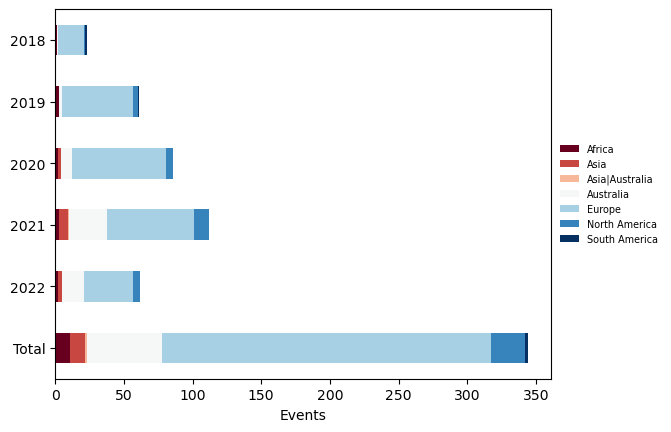
\includegraphics[width=\textwidth]{images/tiaas-events-per-year.png}
         \caption{Events per year and continent}
         \label{fig:tiaas-events-per-year}
    \end{subfigure}
    \hfill
    \begin{subfigure}[b]{0.45\textwidth}
         \centering
         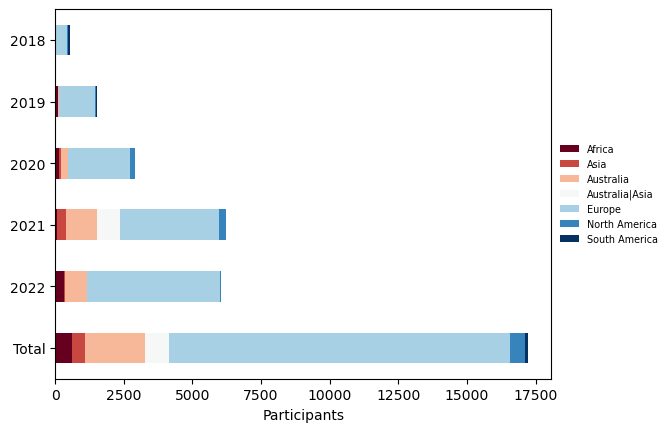
\includegraphics[width=\textwidth]{images/tiaas-participants-per-year.png}
         \caption{Participants per year and continent}
         \label{fig:tiaas-participants-per-year}
    \end{subfigure}
    \hfill
    \begin{subfigure}[b]{0.45\textwidth}
         \centering
         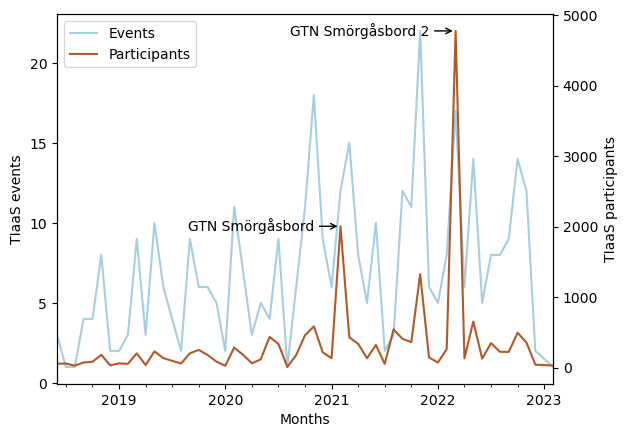
\includegraphics[width=\textwidth]{images/tiaas-events.png}
         \caption{Events and participants over months}
         \label{fig:tiaas-events}
    \end{subfigure}
	\caption{Usage of the TIaaS (Training Infrastructure as a Service) from the European Galaxy server over the months.}. 
	\label{fig:tiaas}
\end{figure}


\bibliography{references}
\end{document}

